\setchapterpreamble[u]{\margintoc}
\chapter{Generation of infrared point clouds}
\labch{thermal_pc}
\label{sec:thermal_pc}

\section*{About this chapter}

This chapter describes the generation of dense thermographic point clouds by mapping image datasets into large \acrshort{rgb} point clouds. The \acrshort{gpu} hardware is used to accomplish these time-consuming tasks with low response time, outperforming currently available approaches for generating thermal point clouds. Occlusion and visibility tests are also addressed for projecting accurate thermal data, together with the use of penalty and aggregation functions. Finally, the generated point cloud is applied to the thermal characterization of vegetation. The complete workflow of this methodology is shown in Figure \ref{fig:thermal_projection_overview}.

The proposed methodology overcomes the current state-of-the-art drawbacks of the reconstruction of thermal point clouds. The solution is implemented from scratch, thus enabling low-level optimizations and taking advantage of \acrshort{gpu} capabilities. Firstly, a baseline point cloud is reconstructed through \acrshort{sfm}-\acrshort{mvs} and high-resolution \acrshort{rgb} imagery. Consequently, large and dense point clouds are the input of the approach that is later explained. Then, co-acquired \acrshort{rgb} and thermal image datasets are registered, and the subsequent projection of a 3D point cloud into the \acrshort{rgb}-thermal image space is performed by addressing the geometric properties of the scene. a viable geometrical description of the scene. Furthermore, the use of several aggregation functions that minimize the distance from aggregated values (3D point cloud) to image samples is evaluated. The outcome is a dense thermal point cloud that preserves image details.

The full source code is available at\newline \small\url{https://github.com/AlfonsoLRz/RGBThermalFusion}.\normalsize

\section{On the generation of thermal point clouds}

Infrared radiation provides valuable data that enable detecting and describing the scene surfaces. Furthermore, the acquisition of high-resolution \acrshort{uas}-based imagery provides an opportunity to estimate highly precise three-dimensional models from a scene, such as point clouds or \acrshort{dsm}. 3D models in Remote sensing are mainly achieved by using laser sensors, e.g., \acrshort{lidar} \cite{yandun_narvaez_survey_2017}, and photogrammetry. Furthermore, 3D representations of surveyed environments have been gaining interest. Firstly, the interaction with 3D environments speeds up the tasks of human operators such as detecting building failures \cite{lin_fusion_2019}. Also, the results of 3D reconstructions are much more valuable and informative for the client counterpart. Finally, it reduces the analysis of multiple datasets into a single one where comparisons are effectively performed. Among 3D representations, point clouds have been significantly preferred over mesh models as they do not involve the reconstruction of surveyed surfaces \cite{park_comparison_2019} into polygons. Instead, a discretized version is provided, though its rendering has been proved to achieve nearly mesh-like results with modern hardware and large point clouds \cite{schutz_rendering_2021}.   

As previously stated in Section \nameref{sec:fundamentals_rs}, \acrshort{sfm} relies on pixel data for finding key points that can be detected in several images. Therefore, estimating 3D point clouds from low-resolution thermal imagery is challenging. First, these present more substantial noise in comparison with \acrshort{rgb} images \cite{sledz_thermal_2018} as well as aberration-induced blurring which causes the spreading of the object radiance. Consequently, the number of extracted tie points in thermography images is smaller, and the resulting 3D point clouds are much sparser and less accurate \cite{jarzabek-rychard_supervised_2020}. The outcome is proven to improve if further calibration is considered \cite{ribeiro-gomes_uncooled_2017}; however, identifying \acrshort{gcp}s in thermography may be challenging because of the material appearance and radiance spreading \cite{javadnejad_photogrammetric_2020}. All these shortcomings also worsen the performance of naive fusion approaches, such as the alignment of \acrshort{rgb} and thermographic point clouds with methods such as \acrshort{icp}. 

Table \ref{table:thermal_pc_attributes} shows the nomenclature of the parameters used in this work. Some of them are calculated by the \acrshort{sfm}-\acrshort{mvs} algorithm, whereas others are extracted from the device specifications.

\begin{figure*}
    \centering
    \caption{Summary of the procedure of this work. \acrshort{sfm}-\acrshort{mvs} and image registration stages build isolated results and thus can be performed in parallel. Thermal information is linked to 3D points using aggregation operators that reduce the error from image samples to the outcome. Occlusion is also considered during this process for assigning thermal data. The visualization of the resulting point cloud is improved by highlighting outliers. Finally, the vegetation is identified and characterized using its temperature. }
    \label{fig:thermal_projection_overview}
    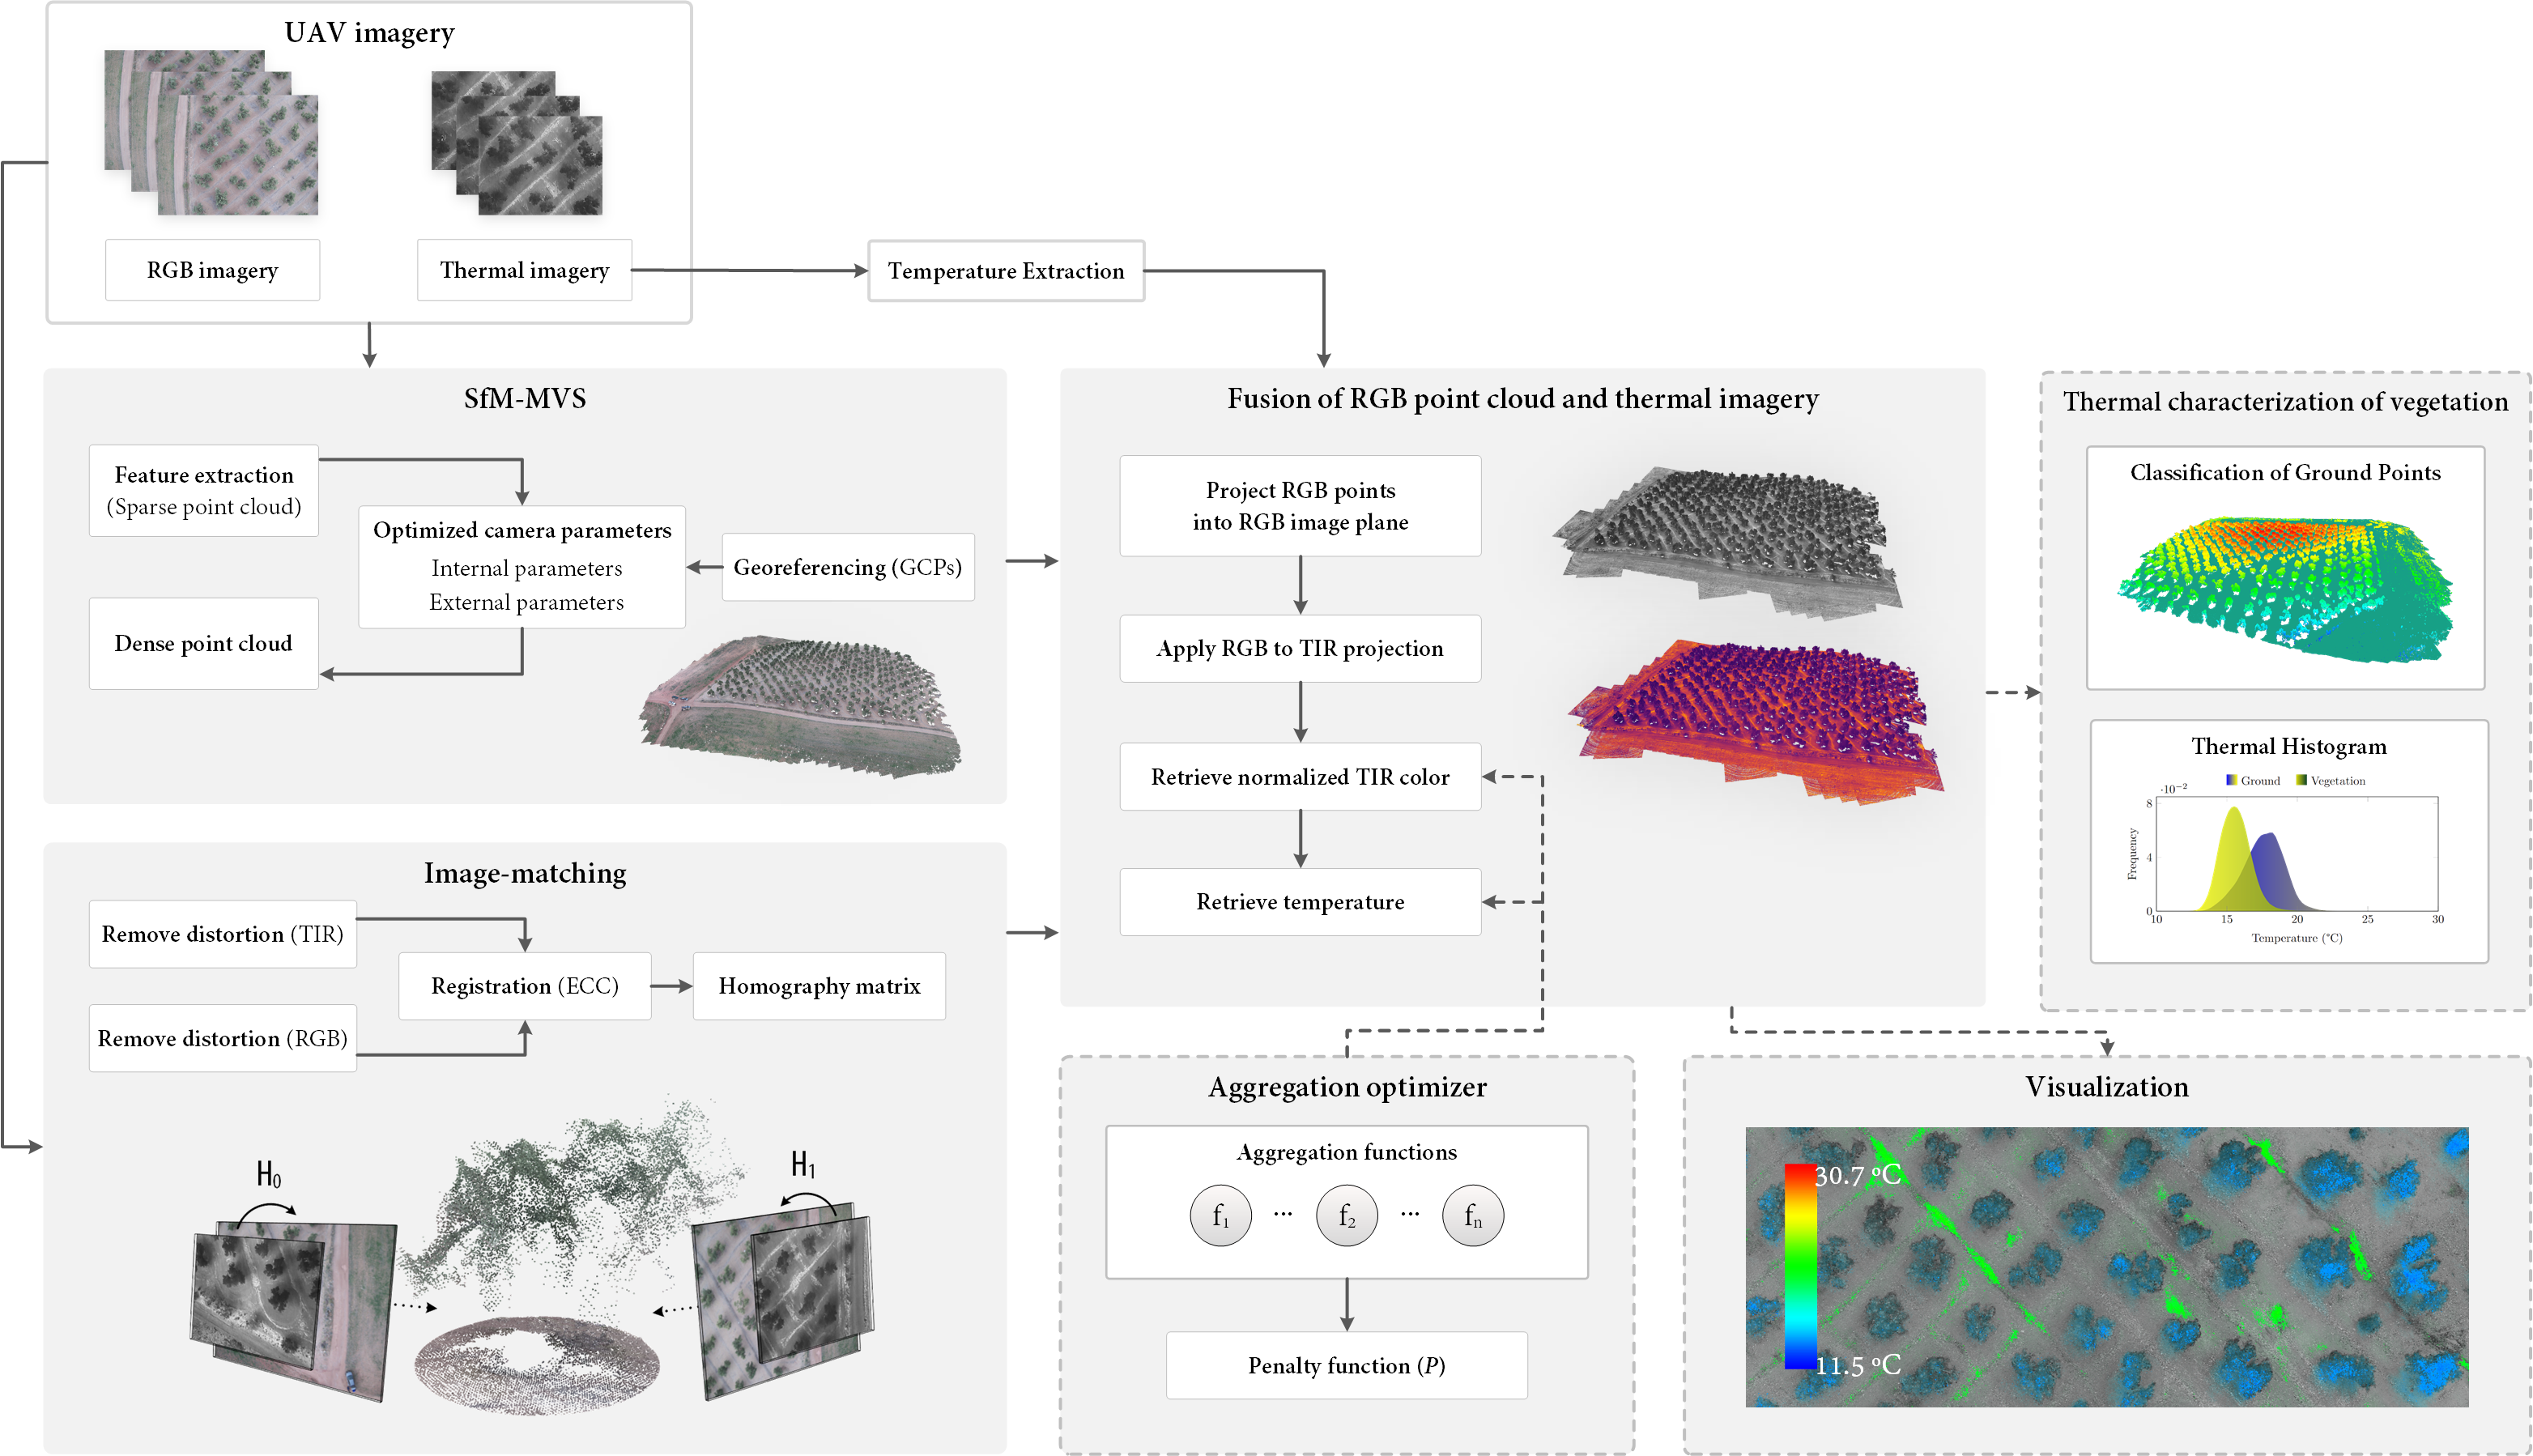
\includegraphics[width=\linewidth]{figs/thermal_projection/thermal_projection.png}
\end{figure*}

\section{Estimation of RGB point clouds}

\acrshort{rgb} point clouds were estimated with \acrshort{sfm}-\acrshort{mvs} using high-resolution \acrshort{rgb} images through methods. Several open-source and commercial software integrate this algorithm and therefore it is trivial to obtain, regardless of the achieved precision. In this work, Pix4Dmapper was used, and the estimation algorithm was further optimized through the marking of \acrshort{gcp}s. The density and storage size of the result depends on the image resolution.

\renewcommand{\arraystretch}{1.15}
\begin{table*}
    \sffamily\small
    \caption{Parameters obtained both from \acrshort{rgb} and thermal camera calibration and image metadata.}
    \label{table:thermal_pc_attributes}
    \begin{tabular}{@{}l@{\hskip 0.55in}l@{}}
    \toprule
    Parameter & Definition\\
    \midrule
    Image size ($w_{\textit{image}}, h_{\textit{image}}$) & Original image size.\\
    Principal point ($c_x$, $c_y$) & Intersection of the principal axis and the image plane. \\
    Focal length ($f_x$, $f_y$) & Distance in pixels from the centre of projection and the image plane. \\
    Sensor width and height ($w_{\textit{sensor}}, h_{\textit{sensor}}$) & Size in millimeters (\si{\milli\meter}). \\
    $\omega, \phi, \kappa$ & Rotation between the image coordinate system and the world system. \\
    Camera position ($t_{\textit{local}}$) & Camera position in the point cloud system.\\
    World offset ($t_{\textit{world}}$) & Offset between the local coordinate system and the UTM system.\\
    Camera matrix ($K$) & Calculated from previous parameters as $\begin{pmatrix} f_x & 0 & c_x\\ 0 & f_y & c_y\\ 0 & 0 & 1\\ \end{pmatrix}$ \\
    Rotation matrix ($R$) & Composite matrix calculated as $R(\omega)R(\phi)R(\kappa)$. \\
    Projection matrix ($P$) & Distortion-free projection in a pinhole model: $K \cdot \begin{bmatrix} R|-Rt_{\textit{local}} \end{bmatrix}$. \\
    Radial distortion coefficients ($k_1, k_2, k_3$) & Distortion coefficients, mostly visible on straight lines.\\
    Tangential distortion coefficients ($p_1, p_2$) & Misalignment of device lens with respect to the image plane. \\
    \bottomrule
    \end{tabular}
    \normalsize
\end{table*}
\renewcommand{\arraystretch}{1}    

\section{Image-matching}

The fusion of \acrshort{rgb} point clouds with thermal data can be performed using the image-matching procedure as a first step. This approach tackles challenges derived from estimating thermal point clouds directly from \acrshort{tir} imagery. Hence, the processing tasks are carried out on a single 3D point cloud, e.g., marking \acrshort{gcp}s. To this end, 3D \acrshort{rgb} points are projected into the \acrshort{rgb} image plane as shown in Equation \ref{eq:thermal_projection}:
\begin{gather}
    \label{eq:thermal_projection}
    \begin{aligned}
        \begin{bmatrix} x^\prime, y^\prime, z^\prime \end{bmatrix}^\intercal = P \begin{bmatrix} x, y, z\end{bmatrix}^\intercal
        \begin{bmatrix} x'', y'' \end{bmatrix}^\intercal = \frac{1}{z^\prime} \begin{bmatrix} x^\prime, y^\prime \end{bmatrix}^\intercal
    \end{aligned}
\end{gather}
provided that $\begin{bmatrix} x, y, z\end{bmatrix}$ is expressed in the local coordinate system where both the point cloud and the cameras are defined. Otherwise, if defined in a global coordinate system such as \acrshort{utm}:
\begin{gather}
    \label{eq:thermal_projection_2}
    \begin{bmatrix} x, y, z \end{bmatrix}^\intercal = \begin{bmatrix} x_{\textit{global}}, y_{\textit{global}}, z_{\textit{global}} \end{bmatrix}^\intercal - t_{\textit{world}}
\end{gather}

Consequently, each 3D point is linked to two values, $x'', y'' \in \mathbb{R}$, for each image. Note that $t_{\textit{world}}$ is defined as an arbitrary shift of real-world points to avoid working with large values. The same reasoning applies to the local positions of cameras, $t_{\textit{local}}$. The matching of \acrshort{rgb} and thermal datasets was achieved using \acrshort{ecc}, thus expressing the misalignment of two images with a homography matrix, $H_i$, of size $3\times3$.

The procedure for applying \acrshort{ecc} to \acrshort{rgb} and \acrshort{tir} images starts by cropping each \acrshort{rgb} image. However, the homography matrix $H_i$ also involves rotations and therefore, the area to be cropped is computed using a rectangle centred at $(\frac{w_{\textit{image}}}{2}, \frac{h_{\textit{image}}}{2})$. It ensures that thermal images are covered by the \acrshort{rgb}'s area of interest in every viewpoint. With this approach, \acrshort{rgb} images are defined as source images, while \acrshort{tir} images are transformed to align both of them. The computed homography matrix projects thermal images into cropped \acrshort{rgb} images as shown in Equation \ref{eq:thermal_projection} and \ref{eq:thermal_projection_2}, whereas the inverse matrix performs the backward projection. 

\begin{marginfigure}[.1cm]
	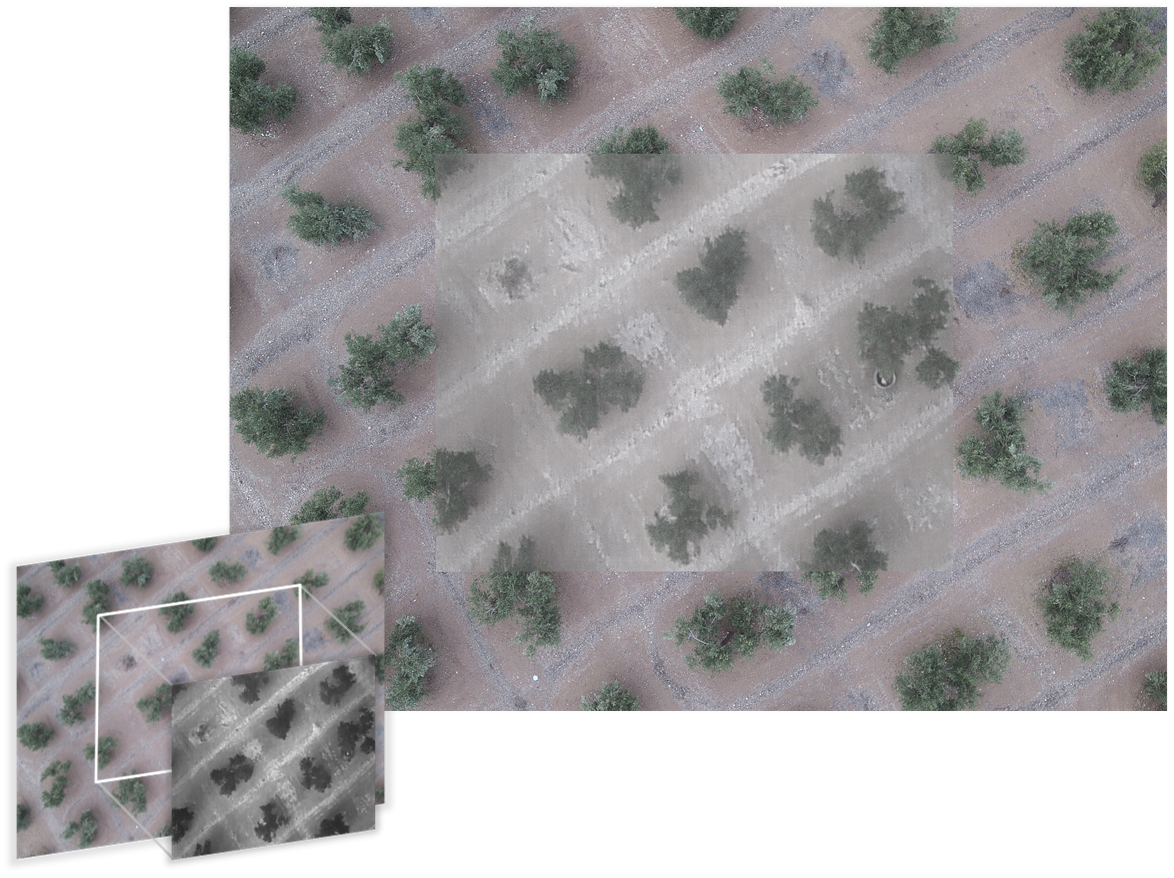
\includegraphics{figs/thermal_projection/thermal_ecc_registration.png}
	\caption{A sample of image-matching between \acrshort{rgb} and thermal images. The latter is overlapped within the \acrshort{rgb} image and depicted with transparency ($\alpha = 0.7$). The bottom image presents the final quadrilateral shape. }
	\label{fig:thermal_ecc_registration}
\end{marginfigure}
In summary, $C_{i} \cdot \inv{H_i}$ projects 2D \acrshort{rgb} points into a thermal image, provided that $C_{i}$ is a composite matrix (Equation \ref{eq:cropping_composite_matrix}) that defines the inverse cropping transformation. Note that projected points may fall out of the thermal image boundaries and a point in polygon test must be carried out. It is very simple to perform in this work since the inverse homography matrix $\inv{H_i}$ leads to an ideal rectangle, and thus only four Boolean operations are required.  
\begin{gather}
    \label{eq:cropping_composite_matrix}
    \begin{aligned}
        C_{i} = & \hspace{1mm} T_{\textit{crop}} * S_{\textit{ratio}} * T_{-\textit{center}_{\textit{\acrshort{rgb}}}} =\\
           = &\begin{bmatrix}
                        1 & 0 & \frac{w_{\textit{thermal}_u}}{2}\\
                        0 & 1 & \frac{h_{\textit{thermal}_u}}{2}\\
                        0 & 0 & 1
                    \end{bmatrix} \cdot 
                    \begin{bmatrix}
                        r_x & 0 & 0\\
                        0 & r_y & 0\\
                        0 & 0 & 1
                    \end{bmatrix} \cdot
                    \begin{bmatrix}
                        1 & 0 & -\frac{w_{\textit{\acrshort{rgb}}_u}}{2}\\
                        0 & 1 & -\frac{h_{\textit{\acrshort{rgb}}_u}}{2}\\
                        0 & 0 & 1
                    \end{bmatrix} =\\
                    = &\begin{bmatrix}
                        r_x & 0 & \frac{1}{2}(-r_{x} w_{\textit{\acrshort{rgb}}_u} + w_{\textit{thermal}_u})\\
                        0 & r_y & \frac{1}{2}(-r_{y} h_{\textit{\acrshort{rgb}}_u} + h_{\textit{thermal}_u})\\
                        0 & 0 & 1
                    \end{bmatrix}\\
        (r_x, r_y) = & \hspace{1mm} \left(\frac{\textit{crop}_x}{w_{\textit{thermal}_u}}, \frac{\textit{crop}_y}{h_{\textit{thermal}_u}}\right)
    \end{aligned}
\end{gather}
where ($\textit{crop}_x$, $\textit{crop}_y$) are the dimensions of the cropped area, ($w_{\textit{thermal}}, h_{\textit{thermal}}$) are the dimensions of undistorted thermal images and \textit{u} subscript refers to the indices of undistorted images. Figure \ref{fig:thermal_ecc_registration} shows the result of the registration methodology as well as the warped quadrilateral shape.

Composite matrices $C_i$ were calculated once and stored in binary files to avoid repeating this time-consuming for every application launch. Some pairs of images may not be matched, and in those cases, the \acrshort{ecc} algorithm either fails to converge or the resulting quadrilateral shape is very distorted. Identifying the second outcome required defining a strict threshold based on the degrees of the minimum/maximum angles after transforming a rectangle shape. Even if some images could not be matched, 3D points were more likely to be visible in multiple images as the drone flight mission was planned with a high overlapping factor. Table \ref{table:image_registration_statistics} shows the percentage of thermal images which could be matched to \acrshort{rgb} images as well as the number of 3D points that were not visible from any registered thermal image. Remark that the \acrshort{fov} is wider for the \acrshort{rgb} device and thus edge points refer to points that were not visible in any thermal images, regardless of the matching results. Hence, it was observed that every unregistered point was not visible from any viewpoint and all of them were located on the edges. For larger point clouds, the number of edge points grows unevenly with respect to the rest of the scenario, thus decreasing the percentage of unregistered and edge points.

\begin{table}
    \sffamily
    \caption{a) Percentage of pairs of \acrshort{rgb}-thermal images that were successfully matched, and b), percentage of points which were not visible from any thermal image for two different point clouds. Edge points refer to points that would not be visible even if the complete image dataset was successfully registered. A large radius ($r \gets 80$\si{\meter}) was utilized during the search of candidate points to avoid omitting visible values.}
    \label{table:image_registration_statistics}
    \begin{tabular}{l@{\hskip 0.3in}l@{}}
        \multicolumn{2}{c}{a) 2D}\\
        \midrule
        \textbf{\#Images} & \textbf{Successfully registered}\\
        \midrule
        410 & 89.7561\% \\
        \bottomrule
    \end{tabular}\\[2mm]
    \begin{tabular}{l@{\hskip 0.3in}l@{\hskip 0.3in}l@{}}
        \multicolumn{3}{c}{b) 3D}\\
        \midrule
        \textbf{\#Points} & \textbf{Not registered points} & \textbf{\#Edge points}\\
        \midrule
        19,161,076 & 18.8952\% & 100\% of 18.8952\%\\
        98,016,324 & 15.5823\% & 100\% of 15.5823\%\\
        \bottomrule
    \end{tabular}
\end{table}

\section{Thermal image mapping}

Merging \acrshort{rgb} and \acrshort{tir} imagery was performed with the previously cited projection. First, a naive approach that neither considered occlusion nor visibility was implemented. As a result, thermal data were mapped to 3D points as long as they were visible from any viewpoint. Equation \ref{eq:thermal_projection} enables projecting each 3D point into the \acrshort{rgb} image plane. Points were considered not visible from a viewpoint and thus discarded if their projected coordinates had values smaller than zero or larger than the dimensionality of \acrshort{rgb} images. In addition, the image matching imposes another rejection condition due to the smaller thermal \acrshort{fov}. 2D coordinates within thermal images ($x_{\textit{thermal}}, y_{\textit{thermal}} \in \R$) were sampled using a bilinear interpolation in which surrounding pixels also affect the outcome. The weight factors were given by their distance to ($x_{\textit{thermal}}, y_{\textit{thermal}}$). The projected values were aggregated using the arithmetic mean as the default approach.

\begin{marginfigure}[.0cm]
	\caption{Rendering of a) an octree whose nodes are spheres, optimized for searches within a radius, and b) a traditional octree whose nodes are boxes. }
	\label{fig:point_cloud_octrees}
	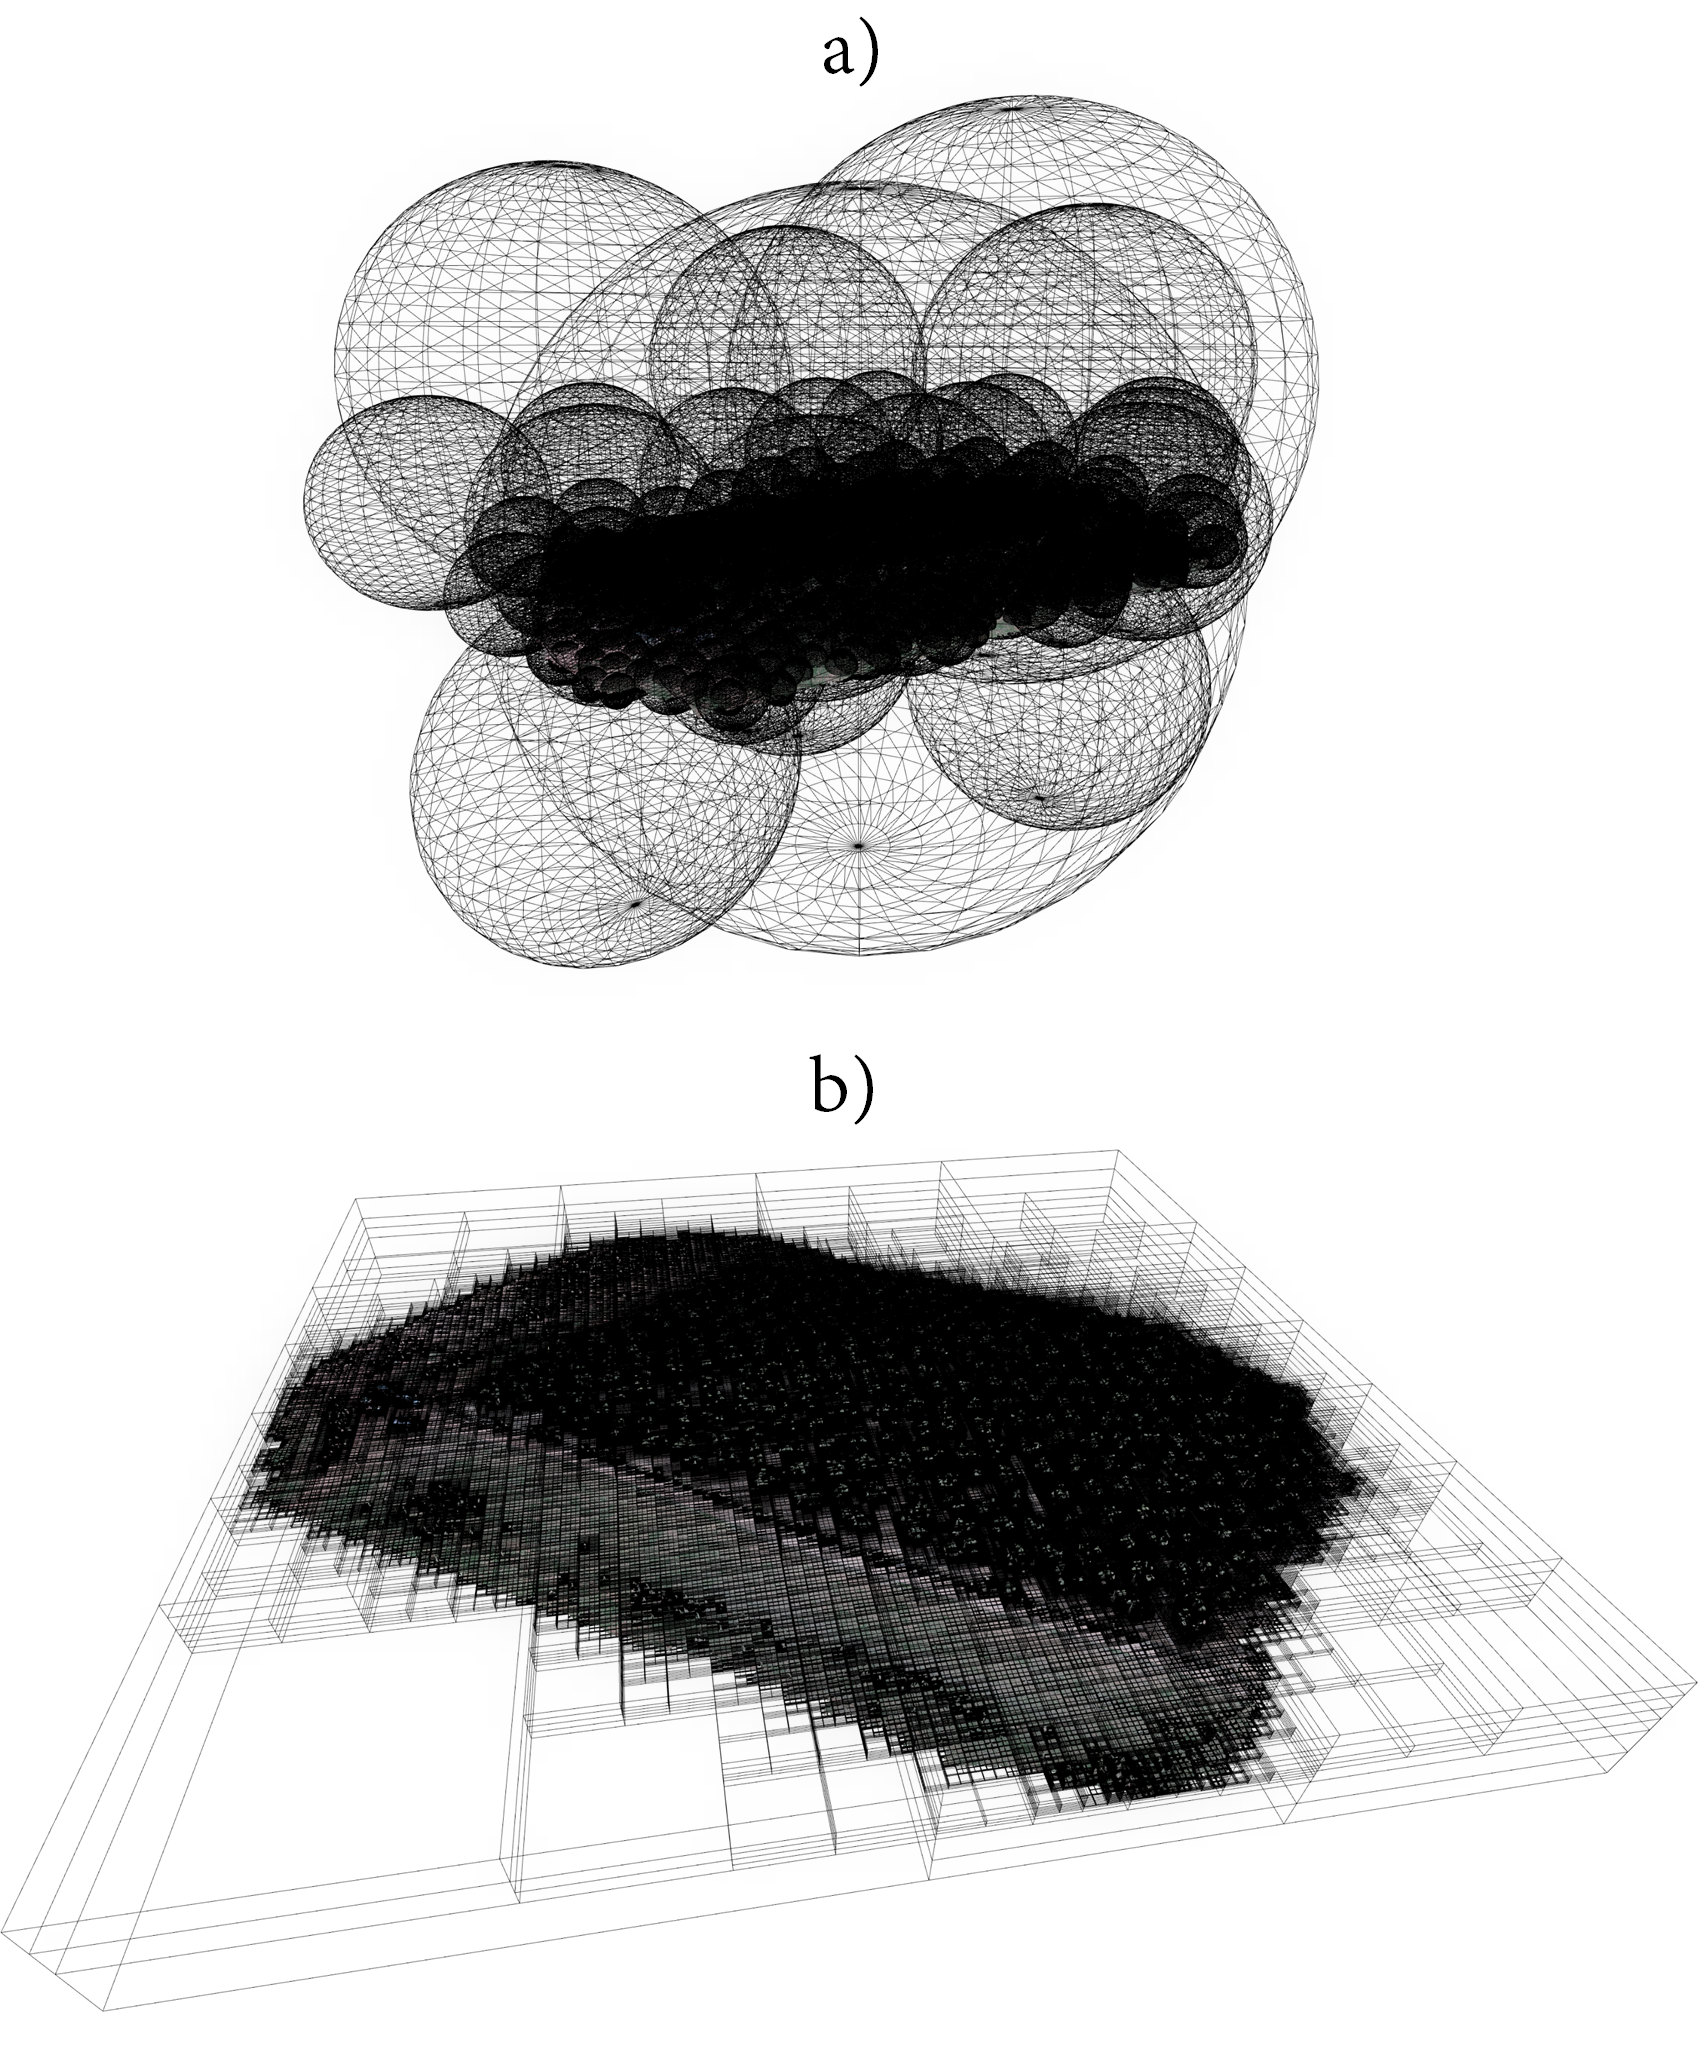
\includegraphics{figs/thermal_projection/octrees.png}
\end{marginfigure}
The main challenge in this stage is to search for candidate points in every image. Points are not assumed to be uniformly sparsed, and therefore, using regular grids is not necessarily the best solution. Indeed, it requires a large memory footprint for fine-grained indexing and efficient searches. Instead, the point cloud was indexed with an octree optimized for searching neighbours within a radius \cite{behley_efficient_2015}. A radius search is preferred over a box search since previous corrections involve interpolations that leave more imprecise values at the boundaries. This data structure indexes 3D \acrshort{rgb} points rather than image viewpoints; otherwise, an efficient search would not be needed due to the relatively low number of images. The search radius is significantly easier to define whether it is expressed at ground level as $(x, \textit{aabb}_{\textit{center}_{y}}, z)$, given that $x$ and $z$ depend on the local position of the image viewpoint and $\textit{aabb}_{\textit{center}_{y}}$ is the $y$-axis coordinate of the central point computed from the scene's \acrshort{aabb}. Figure \ref{fig:point_cloud_octrees} renders the described data structure and a conventional octree. Finally, Figure \ref{fig:thermal_point_cloud_top_view} shows a top view of the reconstructed thermal point cloud.

\begin{figure}[ht]
	\centering
	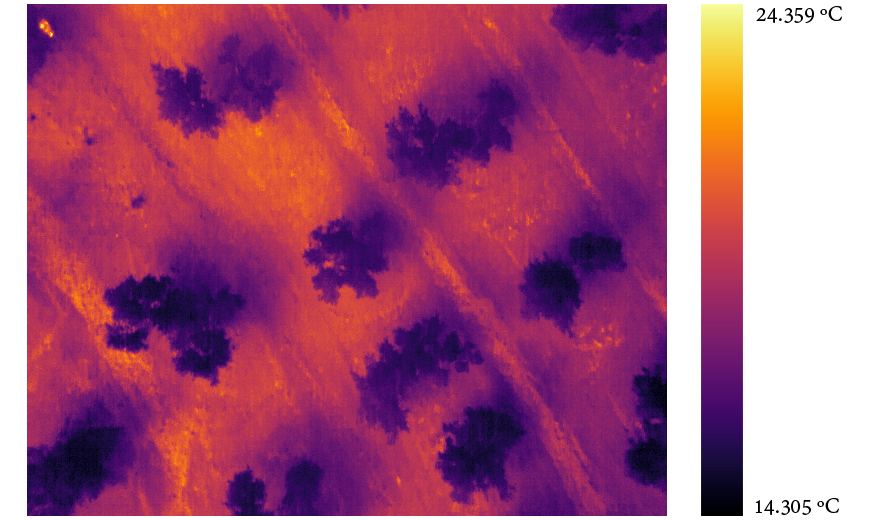
\includegraphics{figs/thermal_projection/thermal_inferno_temperature.png}
	\caption{Top view of a thermal point cloud captured by a \textit{nadir} camera. Absolute temperature values are normalized and mapped to the upper texture. The search radius was fixed to 30 \si{\meter}.}
	\label{fig:thermal_point_cloud_top_view}
\end{figure}

\section{Occlusion}

Although the previous methodology presents a valid and comprehensible approach for reconstructing thermal point clouds, it is theoretically inaccurate. To obtain a more precise projection, occluded points must not obtain data from foreground objects. Occlusion tests have been previously solved by ray-casting voxelized environments; however, this solution lacks accuracy and flexibility since octrees are mainly constructed with top-down methodologies. Therefore, the size of a voxel depends on the subdivision of the point cloud's \acrshort{aabb}, either using a maximum depth or a maximum number of primitives in a single node. At least two approaches are following proposed to solve this challenge. Both lead to point clouds where the amount of thermal information to be aggregated over each 3D point is lower, although these are ensured to be more valuable and precise.

\subsection{Visibility test}

\begin{marginfigure}[-2.0cm]
	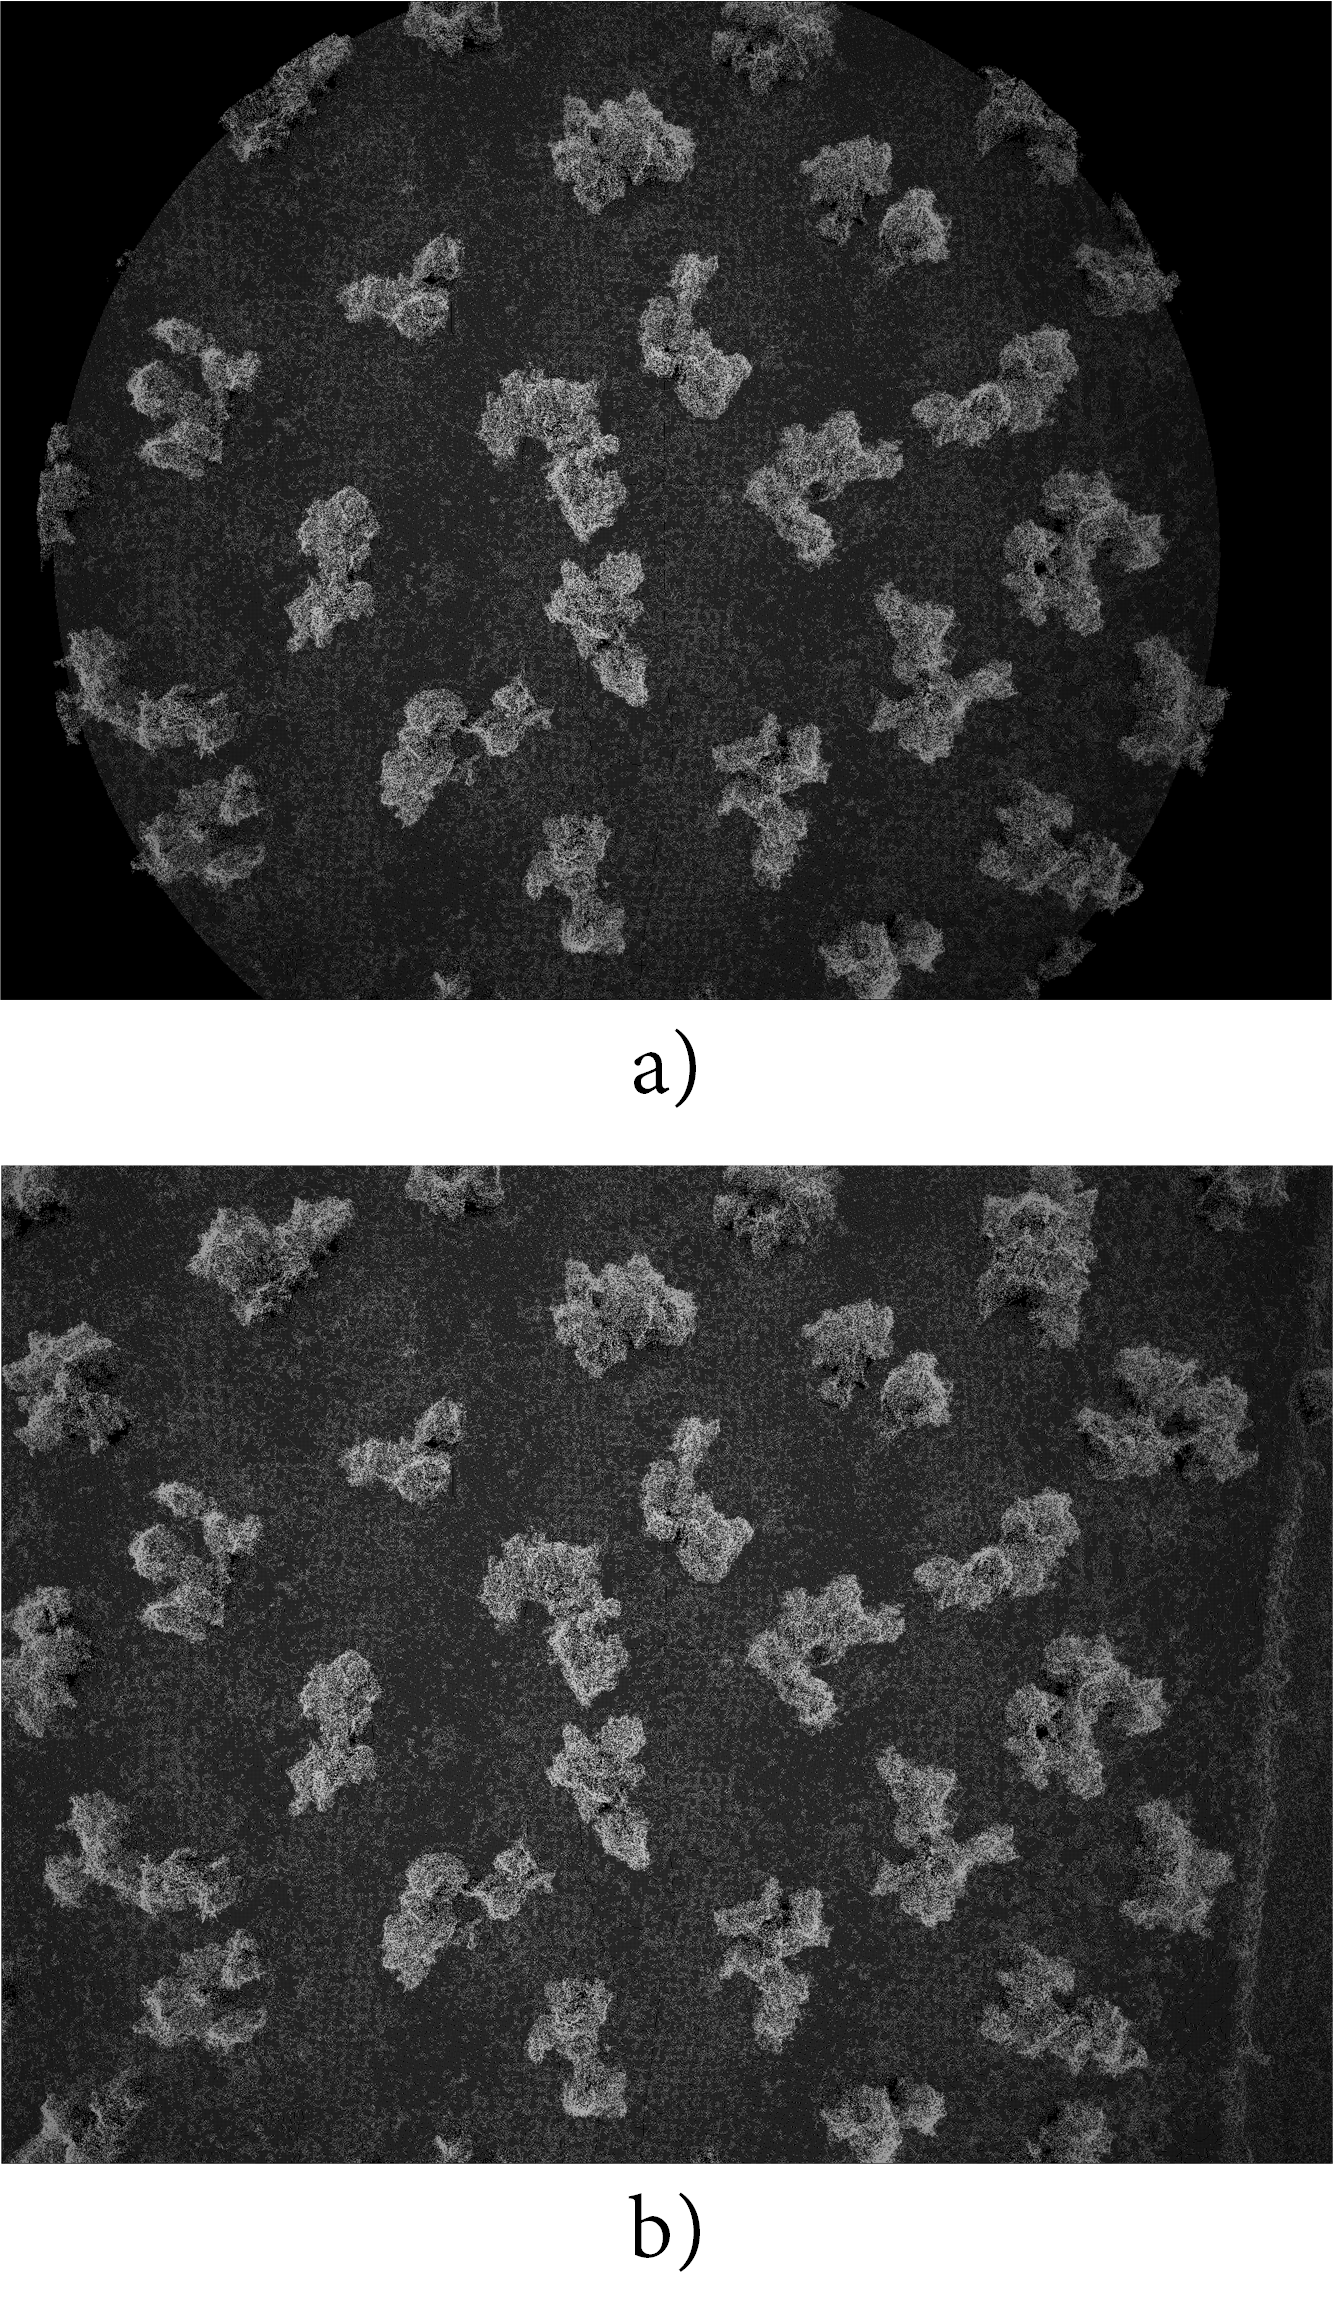
\includegraphics{figs/thermal_projection/depth_buffer.png}
	\caption{Depth buffer of a camera during a visibility test carried out with a radius of size a) 20 \si{\meter} and b) 30 \si{\meter}.}
	\label{fig:depth_buffer}
\end{marginfigure}
Images are discrete representations from where the \acrshort{sfm}-\acrshort{mvs} algorithm can estimate at least one 3D point from every \acrshort{rgb} pixel. A depth buffer (or \textit{z}-buffer) of the same size as the resolution used during the point cloud estimation can be constructed for each image. Still, this size can be increased to build a sub-pixel level method. In this approach, the index of the closest 3D point is stored for every viewpoint and pixel, along with the minimum depth ($\textit{z}$). The latter determines if a point could be visible. Depth buffers were represented as sparse matrices to reduce the memory footprint and implemented as a hash map that stores pairs of values. Keys were the access index of a 2D point and values represented the nearest point for such a position. A depth buffer is depicted in Figure \ref{fig:depth_buffer}, showing a circular pattern as a result of the search algorithm. The workflow for determining which points are visible is presented in Algorithm \ref{alg:depth_buffer_test}.  

\begin{algorithm}
    \small
	\caption{Visibility test to project thermal data into an \acrshort{rgb} point cloud. }
	\label{alg:depth_buffer_test}
    \begin{algorithmic}[1]
        \State \textbf{Input} \acrshort{rgb} point cloud: $P$
    	\State \textbf{Input} \acrshort{rgb} images: $c$
    	\State \textbf{Input} \acrshort{rgb} resolution during \acrshort{sfm}-\acrshort{mvs} procedure: ($w_{\textit{\acrshort{sfm}}}, h_{\textit{\acrshort{sfm}}}$)
    	\State \textbf{Input} Search radius: $R$
        \State \textbf{Output} Array of normalized and absolute temperature
		\For {Every image $c_i$ captured from the position $p_{c_{i}}$}
		    \State Create a new buffer of size ($w_{\textit{\acrshort{sfm}}}, h_{\textit{\acrshort{sfm}}}$) with $d_{x,y} \gets \infty$, provided that $0 \leq x < w_{\textit{\acrshort{sfm}}}$ and $0 \leq y < h_{\textit{\acrshort{sfm}}}$.
		    \State Retrieve candidate points within the radius \textit{R} from the octree
		    \For {Every 3D candidate point $p_j$}
		        \State Calculate 2D \acrshort{tir} point $(x, y)$ (Eq.: \ref{eq:thermal_projection})
		        \If {$(x, y)$ in \acrshort{tir} polygon}
		            \If {$\lVert p_{c_{i}} - p_j \rVert < d_{x, y}$}
		                \State Add point to the depth buffer and update distance at $d_{x, y}$
	    	        \EndIf
	    	    \EndIf
		    \EndFor
		    \For {Every point $p_j$ stored in depth buffer}
		        \State Accumulate normalized and absolute temperature from $c_i$ for $p_j$
		    \EndFor
		\EndFor
		\State Calculate results for each point from $P$ as an arithmetic mean %\;
	\end{algorithmic} 
    \normalsize
\end{algorithm}

\newpage
\subsection{Occlusion test}

\begin{marginfigure}[.0cm]
	\centering
	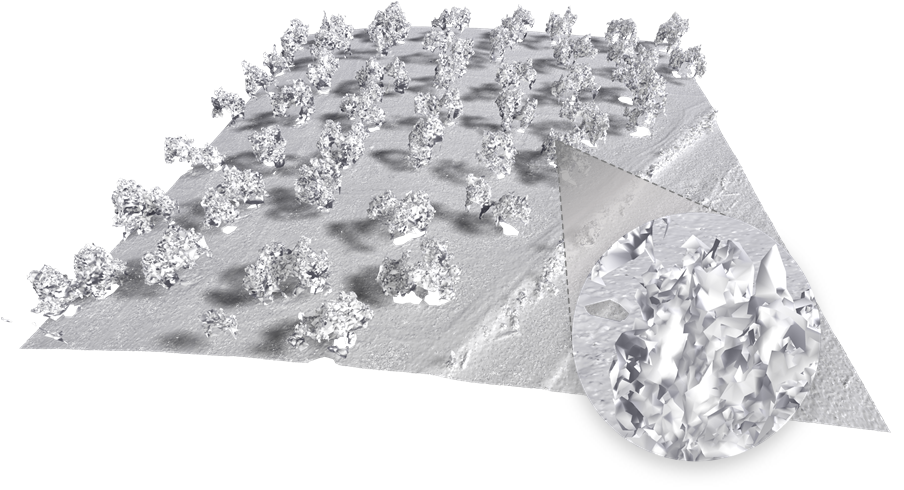
\includegraphics{figs/thermal_projection/triangle_mesh_reconstruction_zoom.png}
	\caption{Triangle mesh estimated for a point cloud subset through Advancing Front algorithm. Reconstruction of vegetation is clearly erroneous in comparison with the ground.}
	\label{fig:advancing_front_mesh}
\end{marginfigure}
Occlusion tests can be performed with ray-casting as long as the target scenario is represented as a triangle mesh. However, estimating the mesh from a point cloud is challenging. Multiple algorithms are found in the bibliography; some require the normal vector, while others are robust enough to work without surface orientation, e.g., the Advancing Front reconstruction \cite{cohen-steiner_greedy_2004}. However, mesh reconstructions are time-consuming and rely on multiple parameters whose values are not trivial to define. Additionally, reconstructing vegetation is more likely to fail since modelling leaves is very intricate. Figure \ref{fig:advancing_front_mesh} shows the result of the Advancing Front reconstruction for a subset of \acrshort{rgb} points. Faces were oriented considering that the viewpoint is above the scene. Hence, faces were flipped if $\hat{n} \cdot \widehat{(v - p)} > \frac{\pi}{2}$, provided that $\hat{n}$ is the surface normal, $v$ is an image viewpoint and $p$ is a 3D point over the triangle mesh surface. A schematic representation of the occlusion methodology is depicted in Figure \ref{fig:occlusion_overview}.

On the other hand, points need a volume to determine whether they are occluded or not. This assumption helps to solve this with ray-casting, and despite being time-consuming, there are data structures optimized for rapidly discarding large parts of the scene, e.g., \acrshort{bvh}s. In this work, volumetric points are modelled using spheres as an efficient alternative to viewpoint-oriented boxes. The radius was computed as a factor relative to the viewpoint altitude (Figure \ref{fig:occlusion_overview}), as shown in Equation \ref{eq:gsd_radius_equation}. It is an efficient yet flexible approach, whereas other shapes, such as an \acrshort{oobb}, require more time-consuming intersection tests.
\begin{equation}
    \label{eq:gsd_radius_equation}
    R = \frac{\frac{w_{\textit{sensor}} \cdot \textit{height}}{f_x \cdot w_{\textit{image}}}}{2} = \frac{\frac{h_{\textit{sensor}} \cdot \textit{height}}{f_y \cdot h_{\textit{image}}}}{2} = \frac{\textit{GSD}}{2}
\end{equation}
with \textit{\acrshort{gsd}} being the size of a pixel if the camera is at an altitude of \textit{height}. \textit{R} is defined in \si{\meter}/pixel, despite $w_{\textit{sensor}}$ and $f_x$ being defined in \si{\milli\meter}.

\begin{marginfigure}[.0cm]
	\centering
	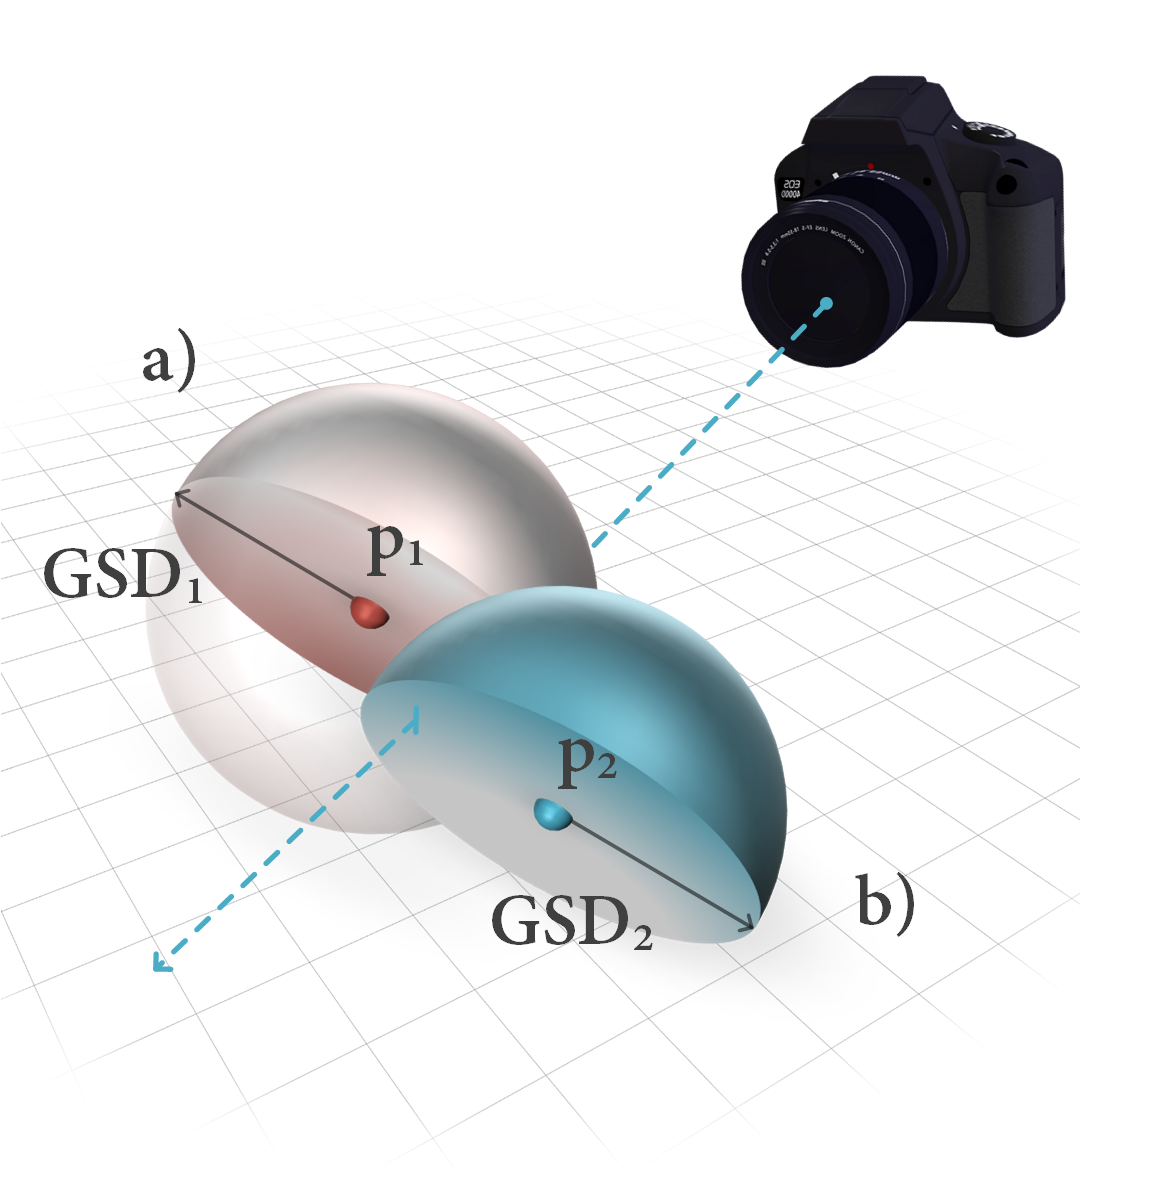
\includegraphics{figs/thermal_projection/occlusion_spheres.png}
	\caption{Occlusion test with two points represented as spherical volumes. a) Point where the ray impacts first ($p_1$), occluding b) the point $p_2$.}
	\label{fig:occlusion_overview}
\end{marginfigure}
Spherical volumes change for each 3D point and image viewpoint and therefore require constructing a different \acrshort{bvh} for every viewpoint and set of points. However, these were constructed using the \acrshort{gpu} hardware as proposed by Meister and Bittner \cite{meister_parallel_2018}. Primitives were ordered using their Morton codes (30 bits representing \textit{xyz} coordinates) and subsequently merged by efficiently searching the nearest neighbour, which also happens to be in a close index of the sorted buffer. On the other hand, the ray-casting was also solved in the \acrshort{gpu} by generating a ray for each 3D point: rays cast from occluded points intersected a closer volume, and those belonging to visible points did not intersect with a closer volume (Figure \ref{fig:occlusion_overview}). The pseudocode of this methodology is illustrated in Algorithm \ref{alg:occlusion_test}.

\begin{algorithm}[hbt]
    \small
	\caption{Occlusion test to determine the temperature of sphere-shaped \acrshort{rgb} points with adaptive radius.}
	\label{alg:occlusion_test}
	\begin{algorithmic}[1]
    	\State \textbf{Input} \acrshort{rgb} point cloud: $P$ %\;
    	\State \textbf{Input} \acrshort{rgb} images: $c$ %\;
    	\State \textbf{Input} Search radius: $R$ %\;
        \State \textbf{Output} Array of normalized and absolute thermal values. %\;
		\For {Every image $c_i$ captured from the position $p_{c_{i}}$}
		    \State Retrieve candidate points within the radius \textit{R} from the octree
		    \State Build a new \acrshort{bvh} with the array of candidate points %\;
		    \Procedure{Sort points}{}
		        \State Sort candidate points expressed as Morton codes and build \acrshort{bvh} leaves %\;
		        \State Join leaf and intermediate nodes while the root is not reached %\;
		    \EndProcedure
		    \For {Every 3D candidate point $p_j$}
		        \State Cast rays from every point and find the nearest intersected volume %\;
		        \If {Intersected volume = $volume_{p_j}$}
		            \State Calculate 2D \acrshort{tir} point $(x, y)$ (Eq.: \ref{eq:thermal_projection}) %\;
		            \If {$(x, y)$ in \acrshort{tir} polygon}
		                \State Accumulate normalized and absolute temperature from $c_i$ for $p_j$ %\;
	    	        \EndIf
	    	    \EndIf
		    \EndFor
		\EndFor
		\State Calculate results for each point from $P$ as an arithmetic mean %\;
	\end{algorithmic}
    \normalsize
\end{algorithm} 

\section{Visualization}

Javadnejad et al. \cite{javadnejad_photogrammetric_2020} visualized thermal point clouds by linearly interpolating \acrshort{rgb} and thermal data. \acrshort{rgb} colours were converted to grayscale and temperature values were mapped to an \acrshort{rgb} value through a colour-ramp function. The weight, $w(t)$, was computed as the distance of each temperature sample, $t$, to the mean, $t_{\textit{mean}}$, so that $w(t) = 1$ omits \acrshort{rgb} colours. Although it accentuates cold and hot regions ($w(t) \gets 1$), intermediate values were also merged with grayscale colours. Therefore, the representation of non-anomalous temperature values distorted the colour distribution of the \acrshort{rgb} point cloud and did not help with the detection of outliers.

Instead, outlier values can be identified using a conventional numeric outlier method. To this end, thermal values were sorted in the \acrshort{gpu} to retrieve first and third quartiles, $Q_1$ and $Q3$, as well as the interquartile range (\textit{IQR} $\gets Q3 - Q1$). Values under $Q_1 - k$(\textit{IQR}) and above $Q3 + k$(\textit{IQR}), where $k \geq 0$, were considered to be anomalous values and thus $w(t)$ was assigned to $1$. The visualization of intermediate values was computed as proposed by Javadnejad et al. \cite{javadnejad_photogrammetric_2020}. However, \acrshort{rgb} colours were not converted to grayscale nor we utilized a linear interpolation. Instead, a Hermite interpolation was used to emphasize values of $t$ close to $t_{\textit{min}}$ and $t_{\textit{max}}$. 

\begin{figure}[ht]
	\centering
	\includegraphics[width=.9\textwidth]{figs/thermal_projection/visualization_thermal_anomalies.png}
	\caption{Visualization of the study area using multiple configurations. a) Visualization proposed by Javadnejad et al. \cite{javadnejad_photogrammetric_2020}, while b), c) and d) show our modified procedure. b) $\gamma = 0.8, k = 0.8$, c) $\gamma = 0.8, k = 0.5$, d) $\gamma = 0.5, k = 0.5$.}
	\label{fig:visualization_thermal_anomalies}
\end{figure}

Equation \ref{eq:blending_function} shows the procedure for computing the proposed enhanced visualization. Note that $\gamma$ enables modifying the brightness of \acrshort{rgb} colours, where $0 \leq \gamma \leq 1$. Figure \ref{fig:visualization_thermal_anomalies} depicts the use of $\gamma$ to darken irrelevant regions. On the other hand, $\zeta(t)$ represents a colour mapping function that is also parameterized by the temperature. In this work, $\zeta(t)$ is given by the texture depicted at the left side of Figure \ref{fig:visualization_thermal_anomalies}.
\begin{gather}
    \label{eq:blending_function}
    \begin{aligned}
        \begin{bmatrix}
            r'\\g'\\b'
        \end{bmatrix} &=
        H(w(t))\zeta(t) + \gamma(1 - H(w(t)))\begin{bmatrix}
            r\\g\\b
        \end{bmatrix}\\
        w(t) &=
        \begin{cases}
            1 &t_{\textit{min}} \leq t < Q_1 - k(\textit{IQR})\\
            \frac{t_{\textit{mean}} - t}{t_{\textit{mean}} - t_{\textit{min}}} &Q_1 - k(\textit{IQR}) \leq t \leq t_{\textit{mean}}\\
            \frac{t - t_{\textit{mean}}}{t_{\textit{max}} - t_{\textit{mean}}} &t_{\textit{mean}} < t \leq Q_3 + k(\textit{IQR})\\
            1 &Q_3 + k(\textit{IQR}) < t < t_{\textit{min}}
        \end{cases}\\
        H(w(t)) &=
        \begin{cases}
            w(t) &w(t) = 1\\
            w(t)^2(3 - 2w(t)) &\text{otherwise}
        \end{cases}
    \end{aligned}
\end{gather}

\section{Aggregation of image samples}

\begin{marginfigure}[.0cm]
	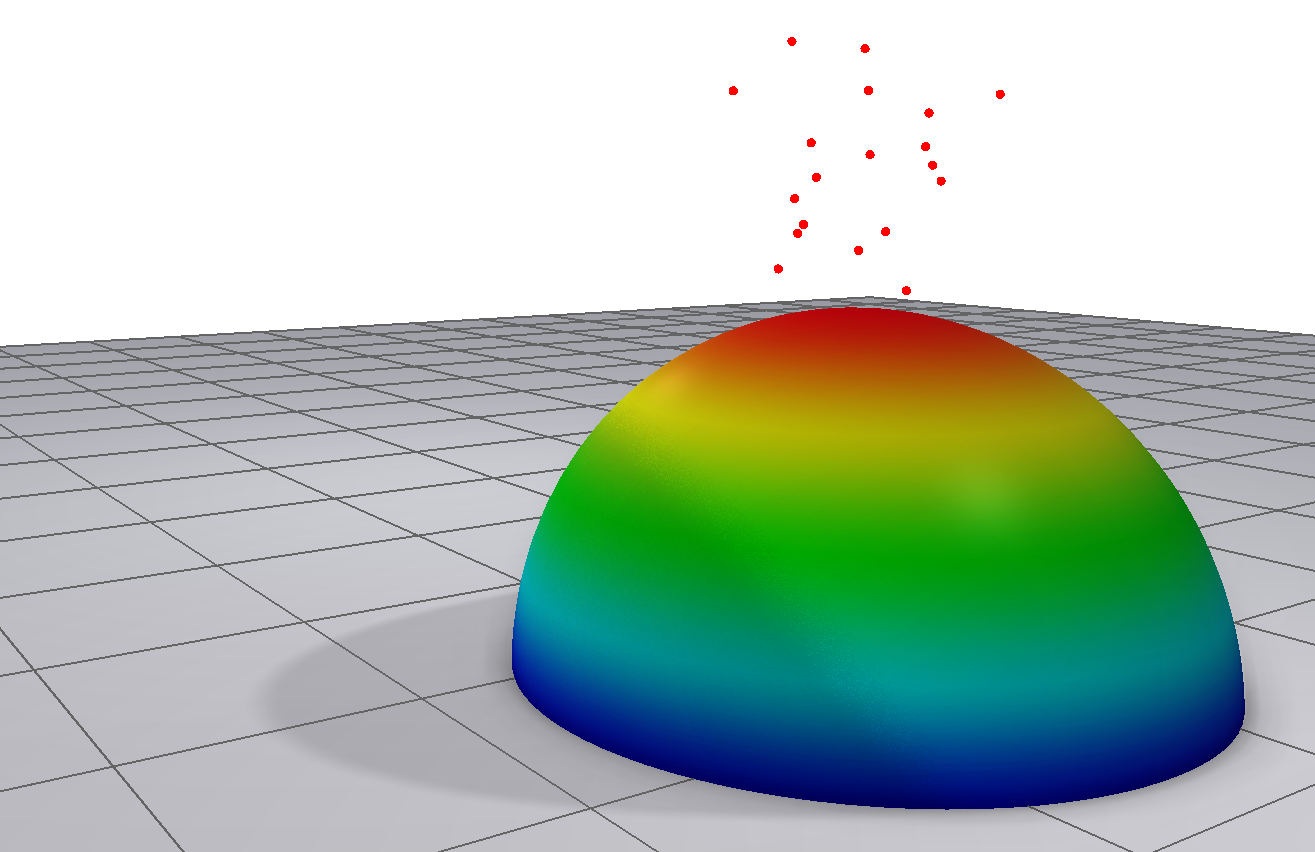
\includegraphics{figs/thermal_projection/brdf_thermal.png}
	\caption{Representation of a point cloud with nineteen \acrshort{tir} radiation samples acquired by different viewpoints from the same point. The semi-sphere represents a Lambertian radiator. }
	\label{fig:brdf_thermal_samples}
\end{marginfigure}
3D points aggregate values from several images that may be different from one another, despite all of them being valid. A frequent shortcut is to average them with the arithmetic mean \cite{javadnejad_photogrammetric_2020} since it is not intrusive at all. However, it is also sensitive to extreme values. Figure \ref{fig:brdf_thermal_samples} depicts nineteen radiation samples that were collected for a single point. Another approach is to use multiple aggregation functions that can be either utilized separately or combined. When combined, their outputs are compared to a set of inputs that help in selecting the aggregation that minimizes the outcome of a penalty function. Consequently, the penalty function determines the similarity of each aggregation output to a set of thermal samples.

The definitions of aggregation operators can be considerably simplified in this work as samples are represented in 1D ($n = 1$). Therefore, we simply needed to define a collection of aggregation and penalty functions, such as the following.
\begin{itemize}
    \setlength\itemsep{0.3em}
    \item Minimum: $f(x) = \underset{i}{\argmin}\, x_i$
    \item Maximum: $f(x) = \underset{i}{\argmax}\, x_i$
    \setlength\itemsep{-0.1em}
    \item Arithmetic mean: $f(x) = \frac{\sum_{i=1}^{n} x_i}{n}$
    \setlength\itemsep{0.85em}
    \item Geometric mean: $f(x) = \sqrt[n]{\prod_{i=1}^{n} x_i}$
    \setlength\itemsep{0.3em}
    \item Harmonic mean: $f(x) = n\left( \sum_{i=1}^{n} \frac{1}{x_i} \right)^{-1}$
\end{itemize}

On the other hand, penalty functions are yet less intricate since their objective is simply to measure the error between the inputs and the aggregated value, $y$. In this regard, three penalty functions \cite{paternain_color_2012} were proposed for minimizing the dissimilarity of aggregations and input samples. 
\begin{itemize}
    \setlength\itemsep{0.5em}
    \item $P_1(x_i, y) = \abs{x_i - y}$
    \item $P_2(x_i, y) = (x_i - y)^2$
    \item $P_3(x_i, y) = \abs{x_i - y}^3$
\end{itemize}

The frequency on which every aggregation function was chosen was monitored for three different penalty functions, $P(x_i, y)$. Table \ref{table:thermal_aggregation_frequency} shows the preference ratio of three local penalty functions against five aggregation operators. The arithmetic mean is the preferred aggregation, despite geometric and harmonic means being also frequently adopted. Maximum and minimum operators were, on the other hand, barely chosen, and their highest frequency was observed for occlusion-based approaches that handle a lower number of samples. From here, the number of operators could be reduced to make this stage more efficient by discarding seldom aggregations.

\renewcommand{\arraystretch}{1.2}
\begin{table*}
    \sffamily\small
    \centering
    \caption{Preference ratio of each aggregation operator over three different penalty functions. Frequency is normalized in $[0, 1]$, and therefore the sum of each row is one. The first and second preferred choices for each configuration are highlighted in bold. }
    \label{table:thermal_aggregation_frequency}
    \begin{tabular}{@{}llccccc@{} }
    \toprule
    & & \multicolumn{5}{c}{\textbf{Aggregation functions}} \\
    \cmidrule{3-7}
    Penalty function & Mapping approach & Arithmetic $\mu$ & Geometric $\mu$ & Harmonic $\mu$ & Maximum & Minimum\\
    \midrule
    \multirow{2}{*}{$g_1 : \underset{y}{\mathrm{argmin}}\, \sum_{i=1}^{n} \abs{x_i - y}$} & Naive & \textbf{0.64699} & 0.07563 & \textbf{0.23348} & 0.02530 & 0.01858 \\
    & Depth buffer & \textbf{0.65672} & 0.06017 & \textbf{0.21589} & 0.03815 & 0.02905 \\
    & Occlusion & \textbf{0.67193} & 0.03362 & \textbf{0.17048} & 0.07004 & 0.05392 \\
    \multirow{2}{*}{$g_2 : \underset{y}{\mathrm{argmin}}\, \sum_{i=1}^{n} (x_i - y)^2$} & Naive & \textbf{0.67787} & \textbf{0.15036} & 0.14783 & 0.01312 & 0.01080 \\
    & Depth buffer & \textbf{0.66193} & 0.13732 & \textbf{0.16330} & 0.02067 & 0.01676 \\
    & Occlusion & \textbf{0.63223} & 0.10407 & \textbf{0.19052} & 0.03972 & 0.03344 \\
    \multirow{2}{*}{$g_3 : \underset{y}{\mathrm{argmin}}\, \sum_{i=1}^{n} \abs{x_i - y}^3$} & Naive & \textbf{0.57092} & 0.14996 & \textbf{0.25392} & 0.01412 & 0.01106 \\
    & Depth buffer & \textbf{0.56471} & 0.13513 & \textbf{0.26142} & 0.02171 & 0.01701 \\
    & Occlusion & \textbf{0.57647} & 0.09821 & \textbf{0.25101} & 0.04057 & 0.03371 \\
    \bottomrule
    \end{tabular}
    \normalsize
\end{table*}
\renewcommand{\arraystretch}{1}

\section{Thermal characterization of vegetation}

Analyzing the temperature of individual surfaces requires segmenting the environment so these can be further studied. The collected datasets comprised a natural environment with soil as well as low and high vegetation, where only the latter two are of interest. A geometric segmentation based on the surface orientation of a point cloud is proposed in this work.

\begin{marginfigure}[1cm]
	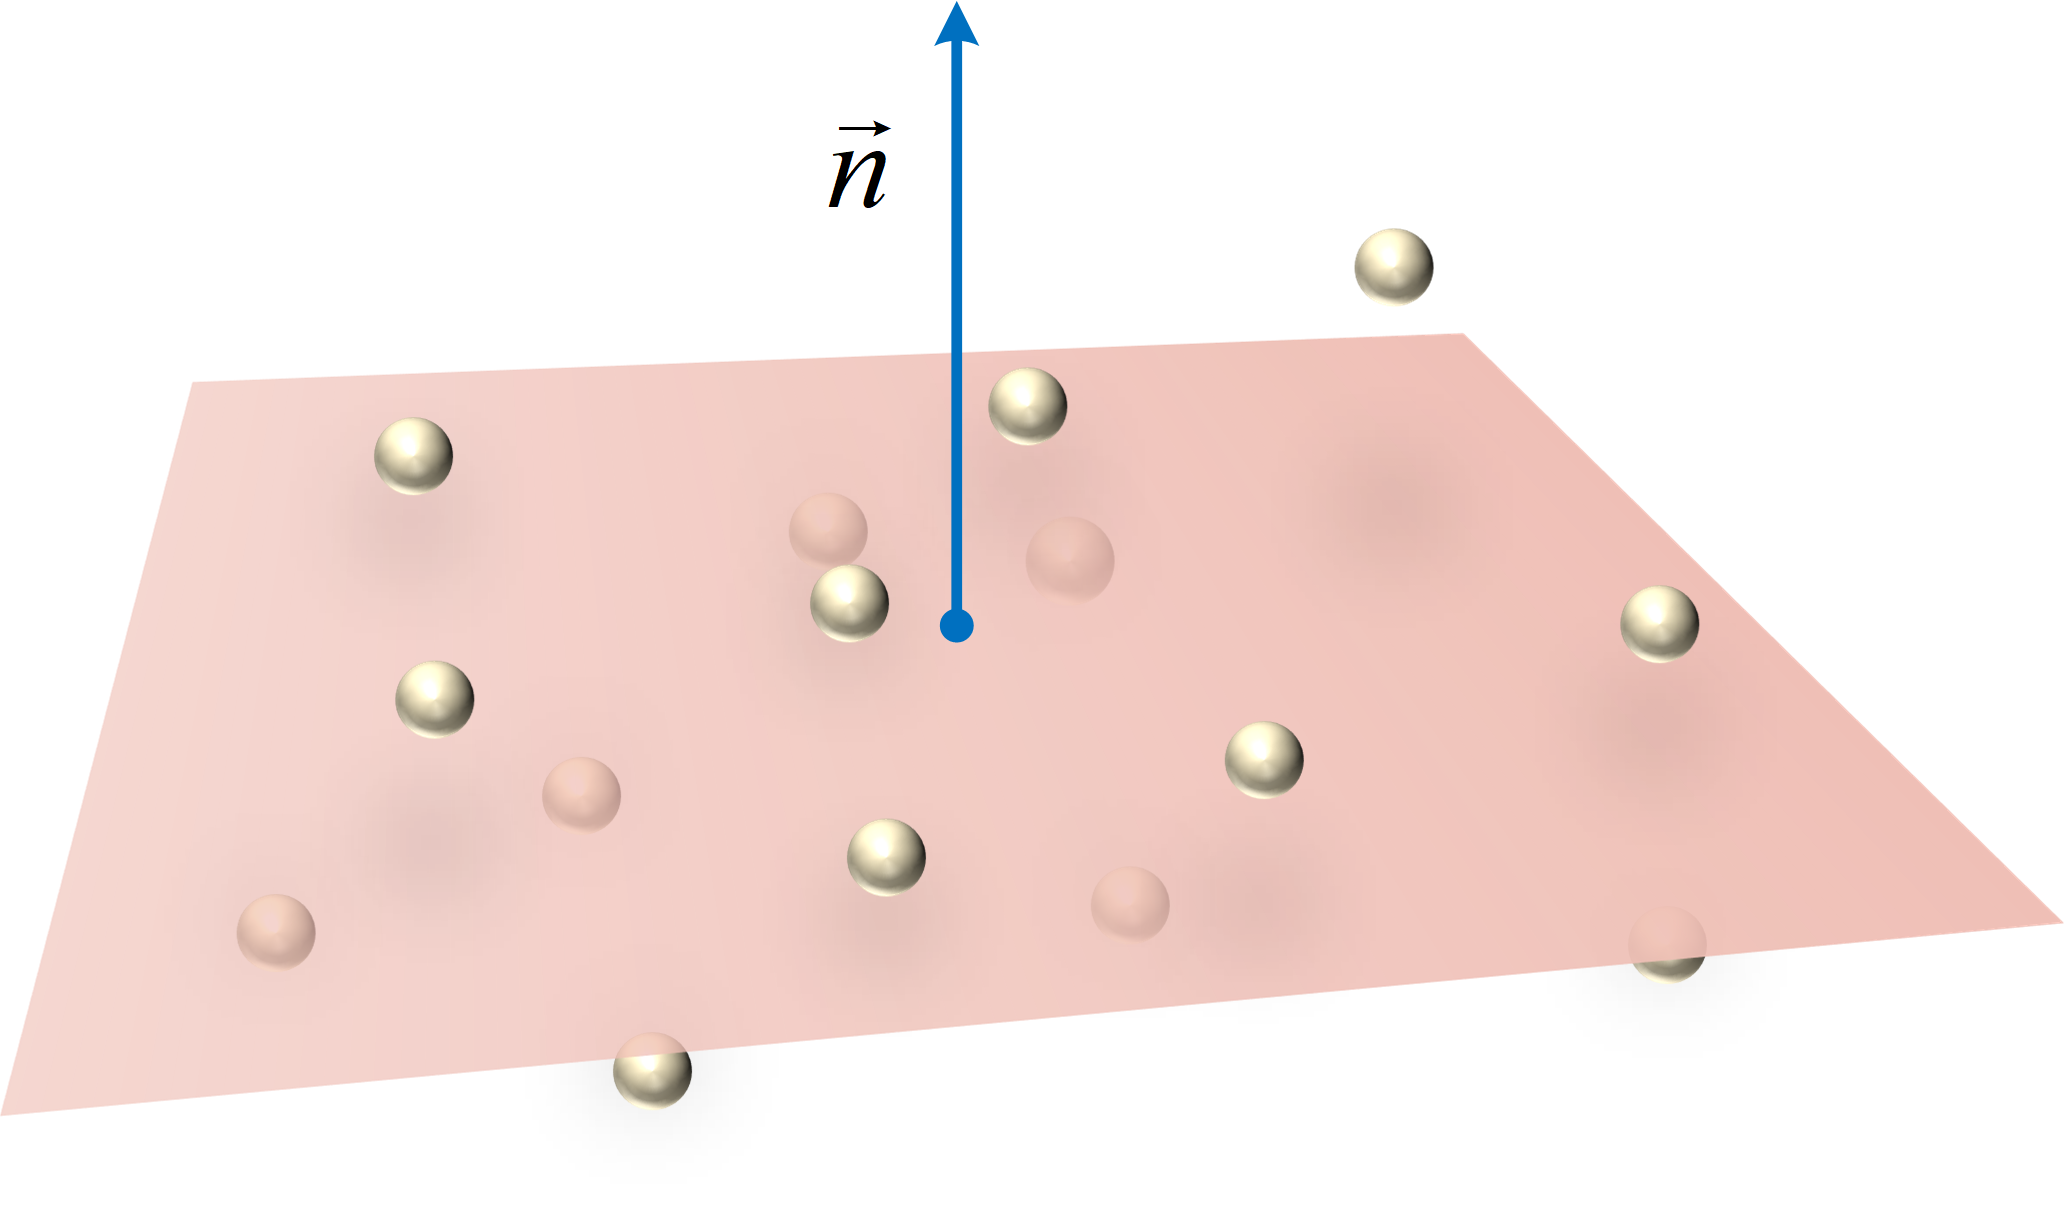
\includegraphics{figs/thermal_projection/plane_fitting.png}
	\caption{Schematic representation of normal estimation by detecting the plane that better represents a group of points.}
	\label{fig:plane_fitting}
\end{marginfigure}
Normal vectors were first computed with several algorithms that will be later compared. Firstly, it can be computed using a \acrshort{knn} search in the \acrshort{gpu}, where the surroundings of a point contribute to its normal estimation. The \acrshort{knn} algorithm can also be optimized with the Morton code sorting: points are spatially ordered along a $\textit{z}$-curve using the Morton encoding and the radix sort algorithm. This solution has been previously explored in high-performance works \cite{jakob_optimizing_2021} since it ensures neighbour searches with linear complexity. These searches are performed over 1D neighbourhoods, where the exploration limit is bounded $2r$, with $r$ being the search radius. Furthermore, the complete search methodology is highly parallelizable in the \acrshort{gpu}, thus allowing us to solve normal estimations in a few minutes at most for large point clouds. Once neighbours are found, normal vectors can be estimated using multiple methods.
\begin{itemize}
    \item First, normals can be computed as the average vector from multiple cross-products calculated between vectors formed by the main point and a neighbour. However, this naïve approach is very sensitive to noise.
    \item A more robust approach is to perform the \acrshort{knn} search and estimate the normal via plane fitting with \acrshort{pca}. It enables estimating the plane that better represents a subset of points \cite{sanchez_robust_2020} using the eigenvector decomposition. As a result, the calculated normal vectors fit better the expected surface (see Figure \ref{fig:plane_fitting}).
    \item Normal estimation is also implemented in open-source libraries, such as Point Cloud Library (\acrshort{pcl}) and the Computational Geometry Algorithms Library (\acrshort{cgal}). \acrshort{pcl} provides \acrshort{cpu} and multi-core \acrshort{cpu} algorithms, whereas \acrshort{cgal} also implements a much slower estimation that was not included in later comparisons.
\end{itemize}

Figure \ref{fig:thermal_normal_estimation} shows a comparison of the response time obtained by the four explained algorithms. The naïve estimation provides baseline results to compare the \acrshort{gpu} implementation, despite both being implemented in the \acrshort{gpu}. As observed, the improved solution has a better performance with larger point clouds, whereas the processing of smaller point clouds offers minor improvements in comparison to the multi-core \acrshort{pcl} implementation. Therefore, the proposed method is proven to be more convenient for large point clouds such as those utilized in this work.

\begin{figure} 
    \centering
    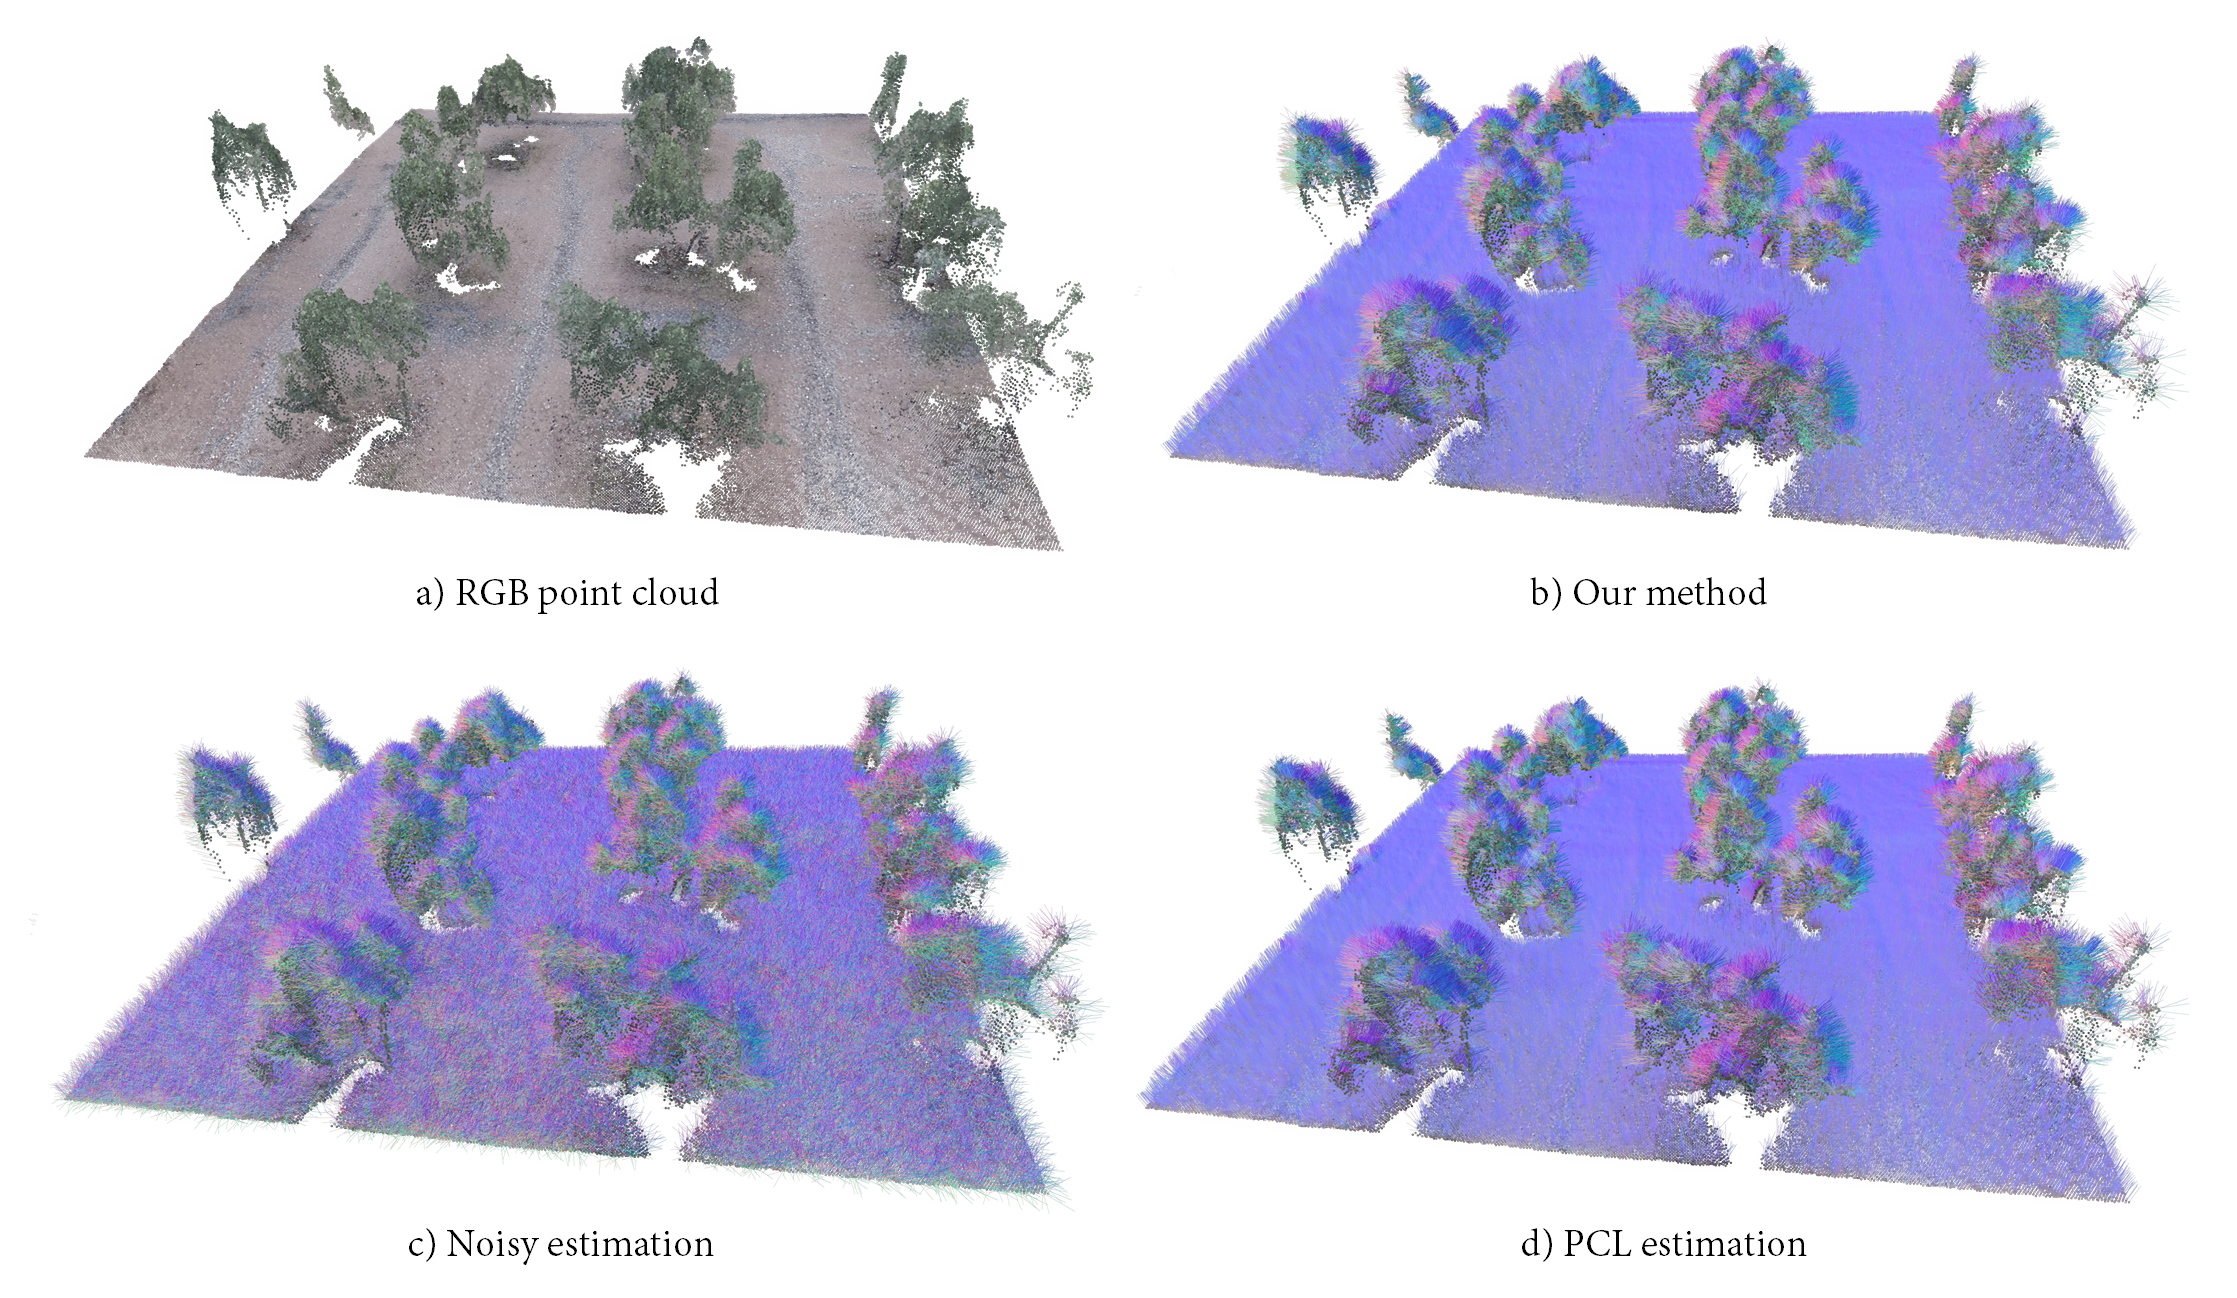
\includegraphics[width=\linewidth]{figs/thermal_projection/normal_estimation.png}
	\caption{Comparison of normal estimation results for a small point cloud. Normal vectors are up-scaled and not normalized to improve the visualization, whereas colours are encoded as the normal vector. The proposed method and \acrshort{pcl} obtain similar results, although ours is more rapid for denser point clouds.}
	\label{fig:thermal_normal_estimation}
\end{figure}

\begin{figure*}
    \centering
    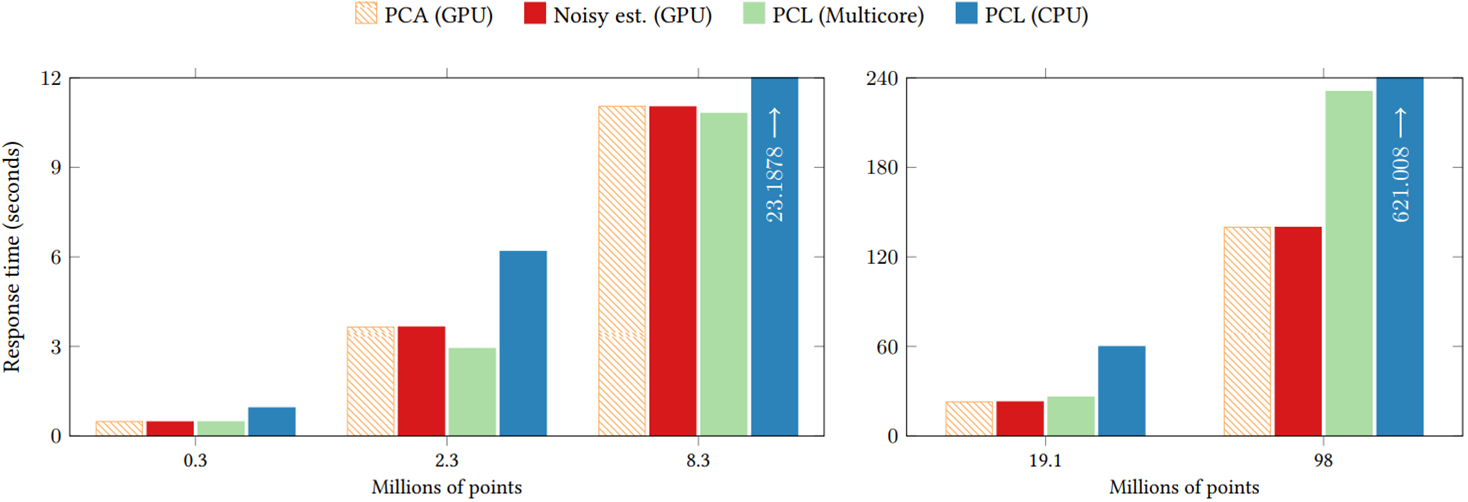
\includegraphics[width=\linewidth]{figs/thermal_projection/response_time_normals.png}
    \caption{Response time, in seconds, measured in the estimation of normals from four different methods. The results were calculated as the arithmetic mean of five different measurements for each algorithm. }
	\label{fig:thermal_normal_response_time}
\end{figure*}

The dot product of the estimated normal vectors, $\hat{n}$, and the $Y$-axis in a Cartesian coordinate system enable separating feasible ground points by defining a threshold, $\hat{n}_{\textit{threshold}}$. Consequently, the complexity of subsequent stages is also reduced, and yet, some ground points remain not filtered. The following step is designed based on the fundamentals of \acrshort{lidar}, where the last returns are more likely to belong to the ground. Again, points were modelled as spheres with a radius $R \gets \frac{\acrshort{gsd}}{2}$ (Equation \ref{eq:gsd_radius_equation}). Still, this method may have some errors as described; points with a slightly higher elevation could prevent detecting surrounding ground points. These false negatives are detected using a tolerance radius, given by $k \cdot \textit{\acrshort{gsd}}$. $k$ is ideally equal to one, i.e., $k \cdot \textit{\acrshort{gsd}}$ is equal to the diameter of spheres. This method is rapidly solved in the \acrshort{gpu} since it first uses the dot product to determine the candidate points, and then, $n$ rays are traced from $p_i + (0, y, 0)$ to $p_i$, provided that $n$ is the number of candidate points and $y$ places the ray's source above the boundaries of the point cloud. Both stages are depicted in Figure \ref{fig:thermal_ground_classification}. 

\begin{kaobox}[frametitle=Application of the proposed classification to other environments]
The proposed method is robust enough for detecting feasible ground points and therefore is designed to work over other kinds of crops. Since it relies on the detection of the last return of a set of traced rays, the method can be configured using a normal vector threshold and a factor, $k$, to scale the sphere radius. This parameterization enables adapting the algorithm to different terrain slopes and point cloud densities.
\end{kaobox}

\begin{figure*}
    \centering
    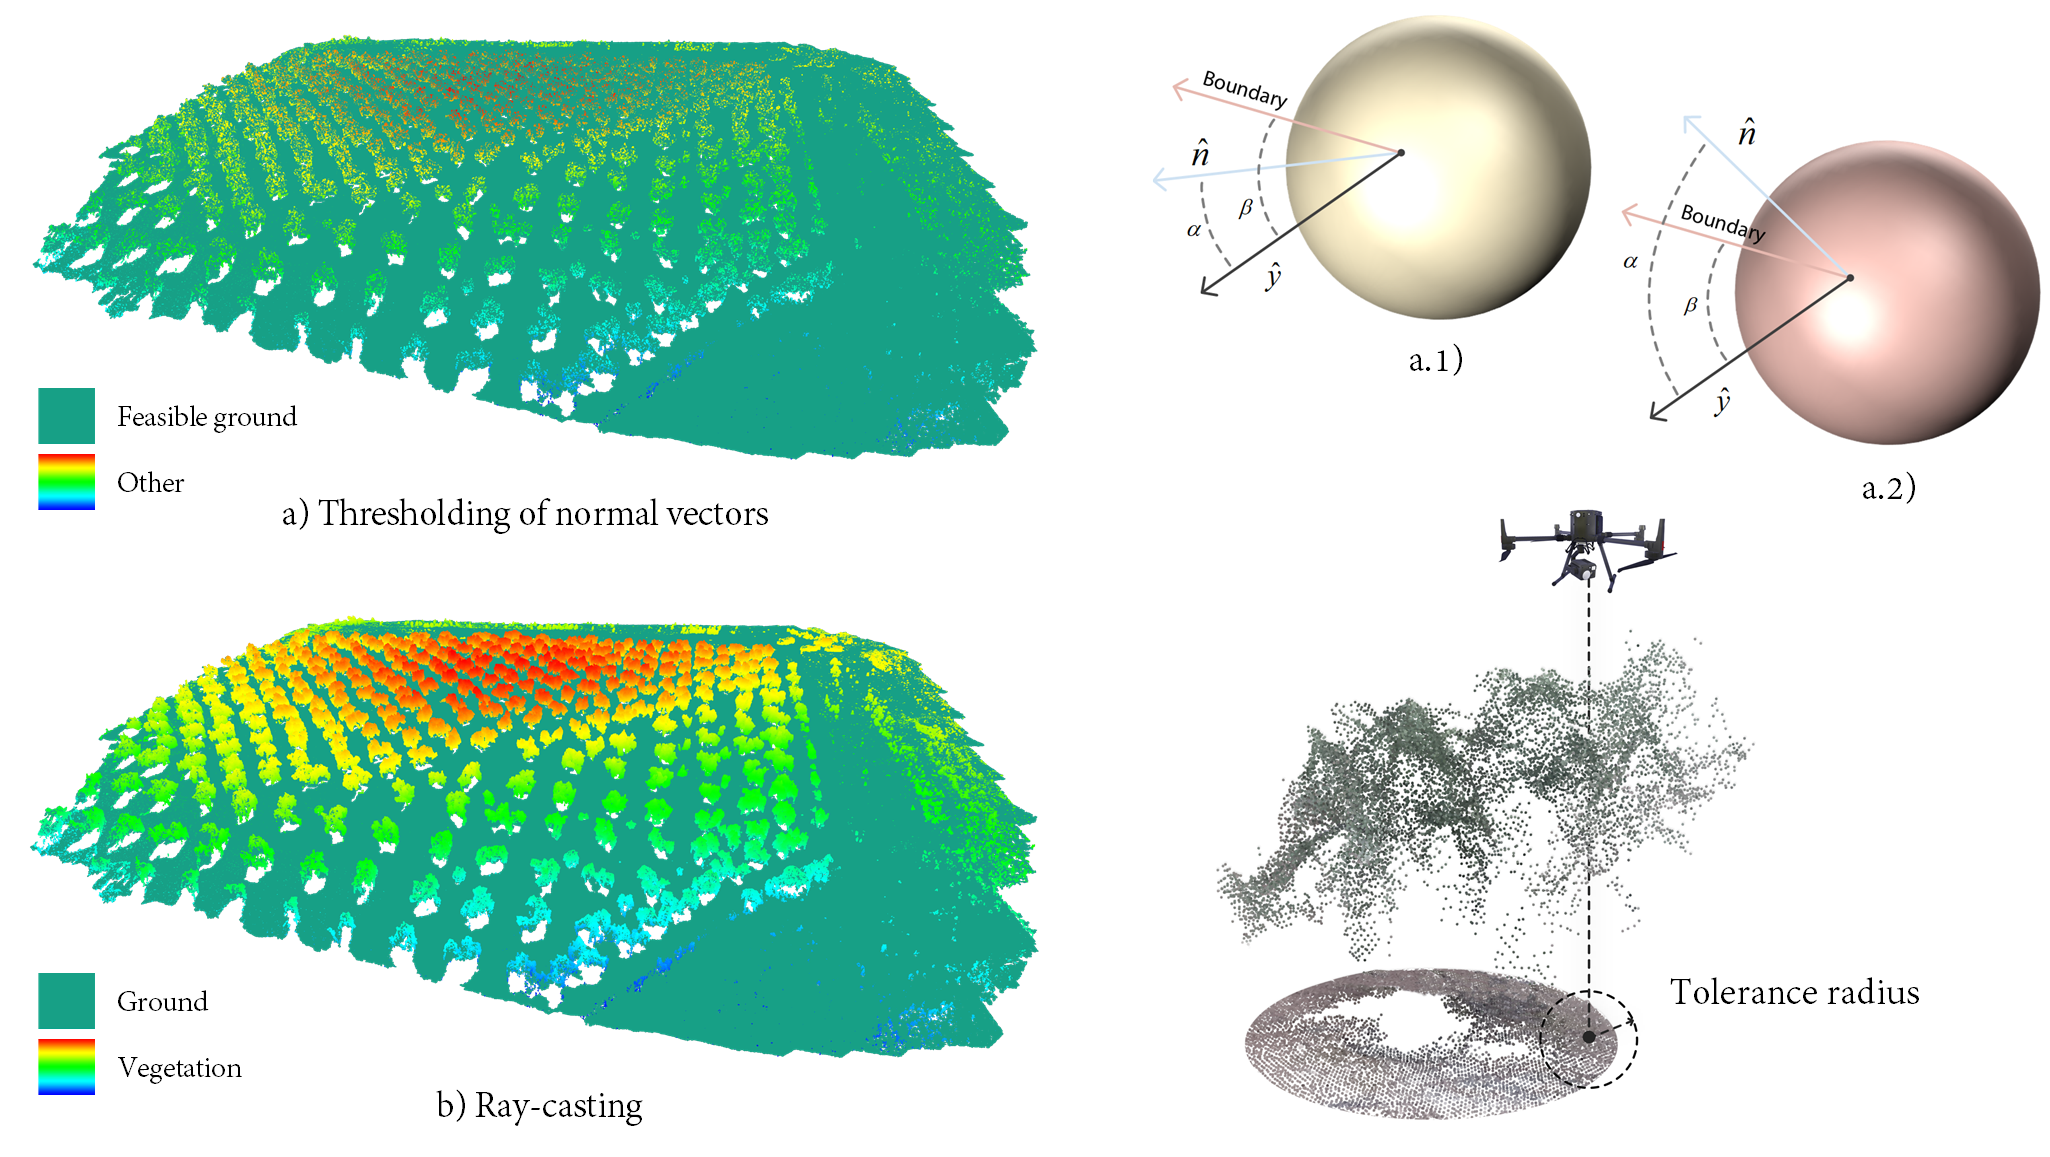
\includegraphics{figs/thermal_projection/thermal_classification_result.png}
	\caption{Classification of ground points with $k = 1$ and a normal threshold of 0,7. a) First step of our methodology, with candidate points being displayed as green points. a.1) Valid candidate point ($\alpha \leq \beta$), a.2) Point discarded for further processing ($\alpha > \beta$). The angles that both normal and boundary vectors form with respect to the $Y$-axis are defined as $\alpha$ and $\beta$ respectively. b) Evaluation of ray-casting for each candidate point. Note that fewer points are rendered as green at this stage. }
	\label{fig:thermal_ground_classification}
\end{figure*}

\section{Results and discussion}
\label{Results and discussion}

The proposed methodology has been checked against three different point clouds of the study area, as depicted in Figure \ref{fig:thermal_study_area}. Therefore, input \acrshort{rgb} point clouds range from 98M points to barely 300k. Comparisons were established with commercial software such as Pix4Dmapper and Agisoft Metashape, and the quality of the results was measured using three key factors: point density, performance and similarity of colour distribution. Hence, the objective is to prove the benefits of the proposed solution in comparison with popular software on the reconstruction of 3D thermal point clouds. Results from third-party software were obtained using the recommended configuration for obtaining the highest \acrshort{lod}, both for aligning images (first phase) and generating a dense point cloud (second phase). Regarding the stochasticity of \acrshort{sfm}-\acrshort{mvs}, it was observed that both Pix4Dmapper and Agisoft Metashape software achieved non-deterministic outcomes and therefore, their results were calculated as the arithmetic mean of five different tests for each solution.

All measurements were performed on a PC with Intel Core i7-7700 3.6 GHz, 16 GB RAM, GTX 1070 \acrshort{gpu} with 8 GB RAM (Pascal architecture) and Windows 10 OS. The proposed methodology is implemented in C++ along with \acrshort{opengl} for rendering. Therefore, parallel algorithms were developed in \acrshort{glsl} (OpenGL Shading Language) using general-purpose compute shaders. 

\subsection{Study area}

The case study is an olive orchard located in Mancha Real (Jaén, Spain), depicted in Figure \ref{fig:thermal_study_area} along with the network of \acrshort{gcp}s. The surveyed area covers  $\sim$ 17,000 \si{\meter\squared}, although reconstructed areas show a larger area due to the sensors' \acrshort{fov}. The ground presents a variable elevation, ranging from 552 \si{\meter} to 572 \si{\meter}. Some of the trees were affected by the pathogen \textit{Xylella fastidiosa}, whose symptoms can be revealed through thermal imagery \cite{zarco-tejada_previsual_2018}. Although this work is not focused on detecting this pathogen, it shows the relevance of estimating a thermal point cloud with reliable radiance. The dataset comprises 820 images; 410 images for each kind of image. Additionally, the network of \acrshort{gcp}s was distributed on the boundaries as well as inside the study area, as proposed by Martínez et al. \cite{martinez-carricondo_assessment_2018}. Also, some of them were placed on points with significant altitude changes.

\begin{figure*}[ht]
    \centering
    \includegraphics[width=\linewidth]{figs/thermal_projection/study_area_overview.png}
    \caption{An overview of the study area. On the left side, the location of the surveyed area in the region of Jaén, whereas the right side shows the polygon of the study area. Coordinates are given in WGS84 (EPSG:4326). The image at the bottom shows three point clouds used throughout this work, from higher to lower size. }
	\label{fig:thermal_study_area}
\end{figure*}

\subsection{Performance of thermal point cloud reconstruction}

An \acrshort{rgb} point cloud of size 98,016,324 was used as the main input to assess the performance of three versions of this work: naive mapping, visibility-based mapping and occlusion-based mapping (solving surface intersections in the \acrshort{gpu}). Commercial software is, on the other hand, fed only with thermographic images. Two different search radii were evaluated: $r_1 \gets 20$ \si{\meter} and $r_2 \gets 30$ \si{\meter}, centred at $y = \frac{\textit{aabb}_{\textit{min}_{y}} + \textit{aabb}_{\textit{max}_{y}}}{2}$ for every image viewpoint, provided that $\textit{aabb}_{\textit{max}_{y}}$ and $\textit{aabb}_{\textit{min}_{y}}$ are the \textit{Y}-axis coordinates of both maximum and minimum points of the point cloud's bounding box. The visibility test is configured so that the size of depth buffers is equal to the size of the original \acrshort{rgb} images ($4000 \times 3000$ px). The occlusion experiment builds \acrshort{bvh}s using Morton codes of 30 bits, sorted with the radix sort algorithm, whereas neighbour searches were performed with a radius of 50. The obtained results are summarized in Table \ref{table:thermal_point_cloud_approaches}. The point cloud area was measured by calculating its convex hull with the Delaunay triangulation \cite{shewchuk_delaunay_2002}. The estimated area was reduced according to the area of internal gaps. Finally, penalty and aggregation functions were omitted during these experiments since further insight will be provided in a later section. 

\renewcommand{\arraystretch}{1.2}
    \begin{table*}
    \sffamily
    \caption{Performance comparison of the proposed methods. The reported values are averaged over five different tests. $r_1$ and $r_2$ correspond to a search radius of 20 \si{\meter} and 30 \si{\meter}, respectively. The best results are highlighted in bold, whereas the number of mapped images shows how many \acrshort{tir} images were successfully projected into the point cloud. Hence, it shows the number of aligned pairs of \acrshort{rgb}-thermal images. For third-party software, some images were excluded whether their parameters could be estimated or no features were detected. }
    \label{table:thermal_point_cloud_approaches}
    \begin{tabular}{@{}lllll@{} }
    \toprule
    & \multicolumn{4}{c}{\textbf{Mapping approach}} \\
    \cmidrule{2-5}
    Attributes & Naive ($r_1$) & Depth buffer ($r_1$) & Occlusion ($r_1$) & Pix4Dmapper\\
    \midrule
    Number of points & 82.743.078 points & 79.511.469 points & 74.181.776 points & 9.782.277 points\\
    Area & 1.9973 ha & 1.9973 ha & 1.9973 ha & 1.9942 ha\\
    Point density & \textbf{4,143 points/\si{\metre\squared}} & 3,981 points/\si{\metre\squared} & 3,714 points/\si{\metre\squared} & 461 points/\si{\metre\squared}\\
    Response time & \textbf{3m 36.54s} & 7m 12.18s & 4m 27.83s & 13m 4.4s\\
    Response time/point & \textbf{2.617 \si{\micro\second}} & 5.435 \si{\micro\second} & 3.61 \si{\micro\second} & 80.185 \si{\micro\second}\\
    Number of mapped images & 368 of 410 & 368 of 410 & 368 of 410 & \textbf{371 of 410}\\[1mm]
    \cmidrule{2-5}
     & Naive ($r_2$) & Depth buffer ($r_2$) & Occlusion ($r_2$) & Agisoft Metashape\\
    \midrule
    Number of points & \textbf{82,767,436 points} & 79,511,469 points & 74,213,254 points & 18,045,885 points \\
    Area & \textbf{1.9991 ha} & \textbf{1.9991 ha} & \textbf{1.9991 ha} & 1.7202 ha \\
    Point density & 4,140 points/\si{\metre\squared} & 3,981 points/\si{\metre\squared} & 3,712 points/\si{\metre\squared} & 1,102 points/\si{\metre\squared} \\
    Response time & 7m 31.01s & 12m 4.38s & 9m 24.92s & 3m 48.31s \\
    Response time/point & 5.449 \si{\micro\second} & 5.435 \si{\micro\second} & 7.61 \si{\micro\second} & 12.113 \si{\micro\second} \\
    Number of mapped images & 368 of 410 & 368 of 410 & 368 of 410 & 326 of 410\\
    \bottomrule
    \end{tabular}
\end{table*}
\renewcommand{\arraystretch}{1}

\subsection{Number of points} 

Thermal point clouds generated with the proposed method have the highest number of points. Despite this metric not reflecting the quality of the result, the geometry was indeed more accurate as it was obtained from an \acrshort{rgb} reconstruction optimized with the marking of \acrshort{gcp}s. In comparison, point clouds reconstructed solely from thermal data have a significantly lower point density. Similarly, the spatial covering is also lower due to the scarce tie-points obtained by \acrshort{sfm}, as reported in Table \ref{table:thermal_point_cloud_approaches} and Figure \ref{fig:thermal_point_cloud_comparison}. The naive approach discards $\sim16$M points which were not visible in any thermal image, whereas the number of points using $r_2$ increased by 358.64\% and 746.09\% with respect to Agisoft Metashape and Pix4Dmapper results. Occlusion-based experiments constructed point clouds of lower size, using a radius equivalent to the \acrshort{gsd}. Still, this approach greatly improved the result of commercial software. On the other hand, incrementing the radius size ($r_2 \rightarrow r_1$) barely improved the number of points, whereas the response time notably increased. Therefore, it can be concluded that $r_1$ is preferred over $r_2$.

\subsection{Area and point density}

The proposed algorithm generated larger results in terms of covered area. Agisoft Metashape had most of its errors at the boundaries, whereas Pix4Dmapper's results were very similar to ours. However, the latter had some gaps within the surveyed area (see Figure \ref{fig:thermal_point_cloud_comparison}). As expected, the larger number of points also provided a higher point density. Hence, the highest point density (from the naive mapping) increased the density by 275.95\% and 798.69\% with respect to Agisoft Metashape and Pix4Dmapper, respectively. As a reference, Javadnejad et al. \cite{javadnejad_photogrammetric_2020} obtained thermal point clouds with a density of 270 points/\si{\meter\squared} (0.36 \si{\hectare} and 95 images), 336 points/\si{\meter\squared} (2.38 \si{\hectare} and 101 images) and 5,429 points/\si{\meter\squared} (0.35 \si{\hectare} and 165 images), while Webster et al. \cite{webster_three-dimensional_2018} operated with thermal datasets of 776 points/\si{\meter\squared}. Note that the point density could be improved by increasing the image overlapping during flight, thus enlarging the dataset dimensionality.

\subsection{Absolute and normalized response time}

The naive approach had the lowest latency, whereas occlusion-based methods were also quite competitive. Remark that Pix4Dmapper and Agisoft Metashape also operate in \acrshort{cuda}-compatible \acrshort{gpu}s. In comparison, the naive and depth buffer approaches were implemented in a sequential manner, while the occlusion-based approach utilized the \acrshort{gpu} to solve intersections. The naive approach shows a small improvement in the overall response time in comparison with Agisoft Metashape, although the normalized response time outperforms commercial software: 78.39\% and 96.73\% less processing time per point with respect to Agisoft Metashape and Pix4Dmapper, respectively. On the other hand, the results from the occlusion mapping with $r_1$ were also remarkable, since this approach requires building a \acrshort{bvh} for every image, each one integrating up to $\sim$6M points ($r_2$ peaks on 14.5 million points). 

\subsection{Aggregation of thermal data}

The proposed methodology was evaluated to check its accuracy in the assignment of thermal values to 3D points. This chapter is relevant for aggregating thermal samples that carry disparate data acquired from different viewing angles. The improvements derived from using penalty functions were assessed by measuring the dissimilarity of aggregated values with respect to the original samples. This distance was evaluated with the \acrshort{rmse}, Mean Absolute Error (\acrshort{mae}) and standard deviation. Note that penalty functions were utilized as local optimizers where a single aggregation operator was selected as the one minimizing the distance, given by a penalty metric. This relation suggests that global metrics are not appropriate to account for aggregation results. Instead, the average \acrshort{rmse} and \acrshort{mae} (Equations \ref{eq:averaged_rmse_mae_avg_01} and \ref{eq:averaged_rmse_mae_avg_02}) criteria fit better for evaluating the quality of the reconstructed thermal values. As a final remark, these metrics are frequently used in unbalanced datasets with only a few items.
\begin{align*}
    &\textit{RMSE}_{\mu} = \frac{\sum_{i=1}^{|P|} \sqrt{\frac{\sum_{j=1}^{|S_i|} (s_j - A_i)^2}{|S_i|}}}{|P|}
    \numberthis \label{eq:averaged_rmse_mae_avg_01}\\
    &\textit{MAE}_{\mu} = \frac{\sum_{i=1}^{|P|} \frac{\sum_{j=1}^{|S_i|} \abs{s_j - A_i}}{|S_i|}}{|P|}
    \numberthis \label{eq:averaged_rmse_mae_avg_02}
\end{align*}
where $i$ refers to the index of a 3D point, $S_i$ is a set of samples linked to such a point, and $A_i$ was the aggregated value. Besides the average metrics, the global \acrshort{rmse} and \acrshort{mae} were annotated in Table \ref{table:thermal_error_dispersion}. \acrshort{rmse} and \acrshort{mae} equations were adapted to point clouds as shown in Equations \ref{eq:rmse_mae_avg_01} and \ref{eq:rmse_mae_avg_02}):
\begin{align*}
    \textit{RMSE} &= \sqrt{\frac{\sum_{i=1}^{|P|} \sum_{j=1}^{|S_i|} (s_j - A_i)^2}{\sum_{i=1}^{p} |S_i|}}
    \numberthis \label{eq:rmse_mae_avg_01}\\
    \textit{MAE} &= \frac{\sum_{i=1}^{p} \sum_{j=1}^{|S_i|} \abs{s_j - A_i}}{\sum_{i=1}^{p} |S_i|}
    \numberthis \label{eq:rmse_mae_avg_02}
\end{align*}

Likewise, the average standard deviation of samples for each 3D point is shown in Equation \ref{eq:average_std}, provided that it does not consider the aggregated value regardless of penalty functions. 
\begin{align*}
    &\sigma_{\textit{mean}} = \frac{\sum_{i=1}^{|P|} \frac{\sum_{j=1}^{|S_i|} \abs{s_j - \{\overline{s_{i_0},...,s_{i_{s_i-1}}}\}}}{|S_i|}}{|P|} 
    \numberthis \label{eq:average_std}
\end{align*}

From the definitions of penalty functions, $P_1$ and $P_2$ (see Table \ref{table:thermal_error_dispersion}), it can be observed that averaged \acrshort{rmse} and \acrshort{mae} are biased towards both functions. However, penalty functions were included to minimize the sample dissimilarity. Despite biases existing towards specific penalty functions,  the metrics show that penalty functions help to reduce the distance from aggregated values to the buffer of image samples. Methods implementing occlusion and visibility tests were expected to have better results for averaged metrics since they have a lower number of samples. However, global \acrshort{rmse} and \acrshort{mae} measured worse results for penalty-based methods since the minimization is applied per point, $S_i$, instead of the overall samples. The best value regarding the averaged \acrshort{rmse} was achieved with the occlusion approach and $P_2$, whereas occlusion together with $P_1$ lowered the dissimilarity measured by the averaged \acrshort{mae}. Nevertheless, penalty-based approaches achieved better results than the alternative baseline, which only used the arithmetic mean. The penalty function $P_1$ minimized the absolute error ($\textit{\acrshort{mae}}_{\mu}$), although $P_2$ and $P_3$ penalized higher changes and therefore minimized $\textit{\acrshort{rmse}}_{\mu}$.

\renewcommand{\arraystretch}{1.2}
\begin{table}[ht]
    \sffamily\small
    \caption{Dissimilarity of aggregated thermal data and 2D thermal samples, without accounting for occluded samples. Errors were computed using values that ranged from 0 to 1. }
    \label{table:thermal_error_dispersion}
    \begin{tabular}{@{}lllllll@{}}
    \toprule
    & & \multicolumn{5}{c}{\textbf{Metric}} \\
    \cmidrule{3-7}
    \textbf{Penalty metric} & \textbf{Approach} & Average $\sigma$ & \acrshort{rmse}$_{\mu}$ & \acrshort{rmse} & \acrshort{mae}$_{\mu}$ & \acrshort{mae}\\
    \midrule
    \multirow{3}{*}{No penalty} & Naive & 0.052 & 0.054 & \textbf{0.052} & 0.045 & \textbf{0.024}\\
    & Visibility & 0.049 & 0.050 & 0.055 & 0.042 & 0.027\\
    & Occlusion & \textbf{0.039} & \textbf{0.042} & 0.054 & 0.042 & 0.054\\
    \midrule
    \multirow{3}{*}{$P_1 : \abs{d(x_i, y)}$} & Naive & 0.052 & 0.054 & 0.053 & 0.044 & \textbf{0.024} \\
    & Visibility & 0.049 & 0.051 & 0.055 & 0.041 & 0.027 \\
    & Occlusion & \textbf{0.039} & 0.042 & 0.055 & \textbf{0.035} & 0.034\\
    \midrule
    \multirow{3}{*}{$P_2 : d(x_i, y)^2$} & Naive & 0.052 & 0.053 & \textbf{0.052} & 0.044 & \textbf{0.024} \\
    & Visibility & 0.049 & 0.050 & 0.054 & 0.042 & 0.027 \\
    & Occlusion & \textbf{0.039} & \textbf{0.041} & 0.053 & \textbf{0.036} & 0.035\\
    \midrule
    \multirow{3}{*}{$P_3 : \abs{d(x_i, y)}^3$} & Naive & 0.052 & 0.054 & \textbf{0.052} & 0.045 & \textbf{0.024} \\
    & Visibility & 0.049 & 0.050 & 0.054 & 0.043 & 0.027 \\
    & Occlusion & \textbf{0.039} & \textbf{0.041} & 0.053 & \textbf{0.037} & 0.035 \\
    \bottomrule
    \end{tabular}
    \normalsize
\end{table}
\renewcommand{\arraystretch}{1}

\begin{figure*}
    \centering
    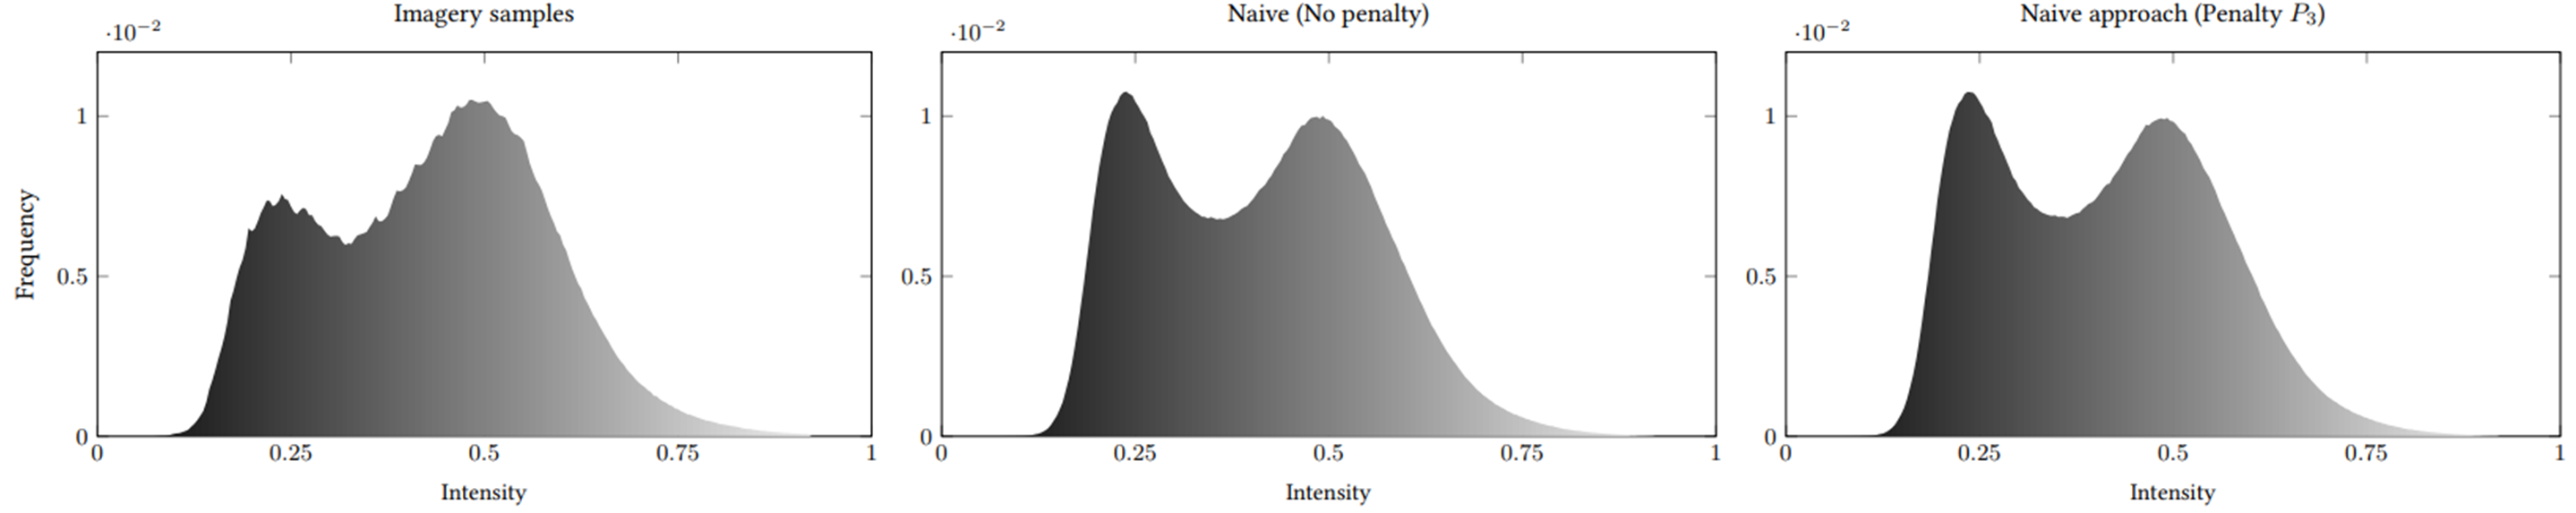
\includegraphics[width=\linewidth]{figs/thermal_projection/density_function.png}
	\caption{Intensity distribution of image samples collected during the reconstruction of a thermal point cloud, as well as the grayscale distribution obtained after using the naive-no penalty) and naive-penalty ($P_3$) approaches. The density functions concerning other variants were omitted as they returned very similar results.}
	\label{fig:thermal_histogram_results}
\end{figure*}

The results from aggregation operators were evaluated by measuring the distance between histograms concerning pixels and 3D points. Despite image samples being very different from each other, penalty functions were evaluated to check whether they produced variations in distance metrics. For that purpose, three conventional criteria were used to compare histograms, ranging from the Pearson \acrshort{cc} (Equation \ref{eq:pearson_correlation}) to the Hellinger distance (Equation \ref{eq:hellinger_distance}) and intersection distance (Equation \ref{eq:intersection_distance}) \cite{cha_comprehensive_2007}. From now on, we will refer to them as $d_{\textit{pearson}}$, $d_{\textit{hellinger}}$ and $d_{\textit{intersection}}$ for the sake of simplicity. $d_{\textit{pearson}}$ coefficient ranges from -1 to 1, with 1 being a perfect correlation. Zero implies there exists no linear correlation and -1 indicates a perfect negative correlation. On the other hand, $d_{\textit{hellinger}}$ measures the similarity of two probability functions, where 1 implies that both distributions are orthogonal. The expression of Equation \ref{eq:hellinger_distance} is simplified if histograms $h_1$ and $h_2$ are defined as density functions in [0, 1] ($h_{\textit{norm}_{1_{i}}}$, $h_{\textit{norm}_{2_{i}}}$). Finally, the intersection, $d_{\textit{intersection}}$, is another widely used form of similarity for probability distributions. It returns 1 when $h_{\textit{norm}_{1_{i}}}$ and $h_{\textit{norm}_{2_{i}}}$ are completely overlapped. 
\begin{align*}
    d(h_1, h_2) &= \frac{\sum_{i=1}^{n} (h_{1_{i}} - \overline{h}_{1}) (h_{2_{i}} - \overline{h}_{2})}{\sqrt{\sum_{i=1}^{n} (h_{1_{i}} - \overline{h}_{1})^2 \sum_{i=1}^{n} (h_{2_{i}} - \overline{h}_{2})^2}}
    \numberthis \label{eq:pearson_correlation}\\
    d(h_1, h_2)
    &=\sqrt{1 - \frac{1}{\sqrt{\overline{h}_1 \overline{h}_2 \textit{n}^2}} \sum_{i=1}^{n} \sqrt{h_{1_{i}}h_{2_{i}}}}\\
    &=\sqrt{1 - \sum_{i=1}^{n} \sqrt{h_{\textit{norm}_{1_{i}}}h_{\textit{norm}_{2_{i}}}}}
    \numberthis \label{eq:hellinger_distance}\\
    d(h_1, h_2)
    &=\sum_{i=1}^{n} \min(h_{1_{i}}, h_{2_{i}})
    \numberthis \label{eq:intersection_distance}
\end{align*}
where $n$ is the number of bins of histograms $h_1$ and $h_2$, both with the same dimensionality.

\begin{figure*}
    \centering
    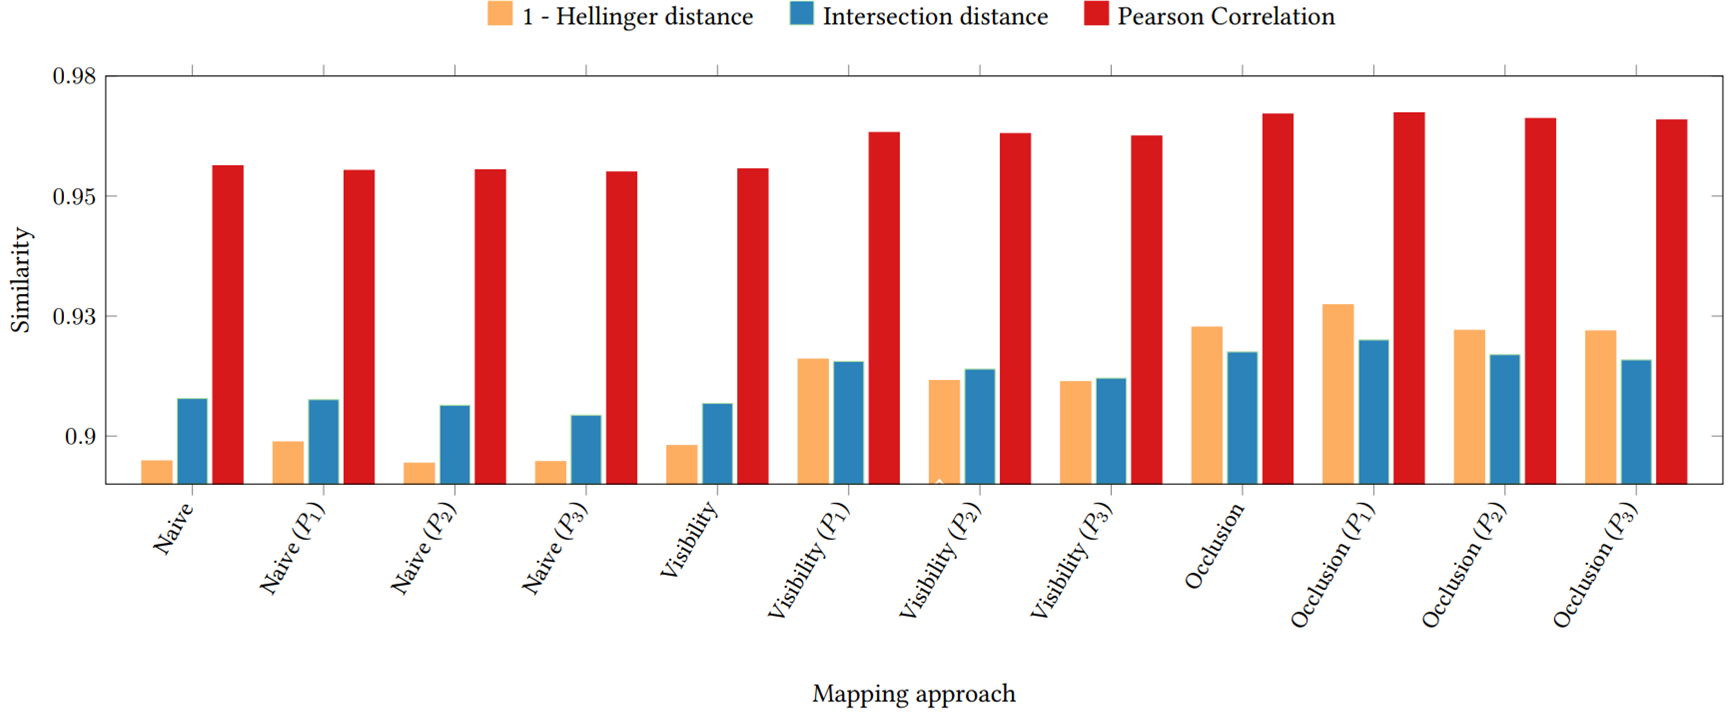
\includegraphics[width=\linewidth]{figs/thermal_projection/distance_similarity.png}
	\caption{Similarity between histograms for each configuration. For the sake of clarity, Hellinger distance was expressed as $1 - d$ to visualize the three metrics in the same chart. Hence, a value of 1 indicates that both histograms are equal ($h_{1_{i}} = h_{2_{i}}, \forall i \in [0, n)$), while 0 denotes complete dissimilarity ($h_{1_{i}} = 1 - h_{2_{i}}, \forall i \in [0, n)$).}
	\label{fig:thermal_histogram_results_02}
\end{figure*}

% \begin{figure*}
%     \centering
%     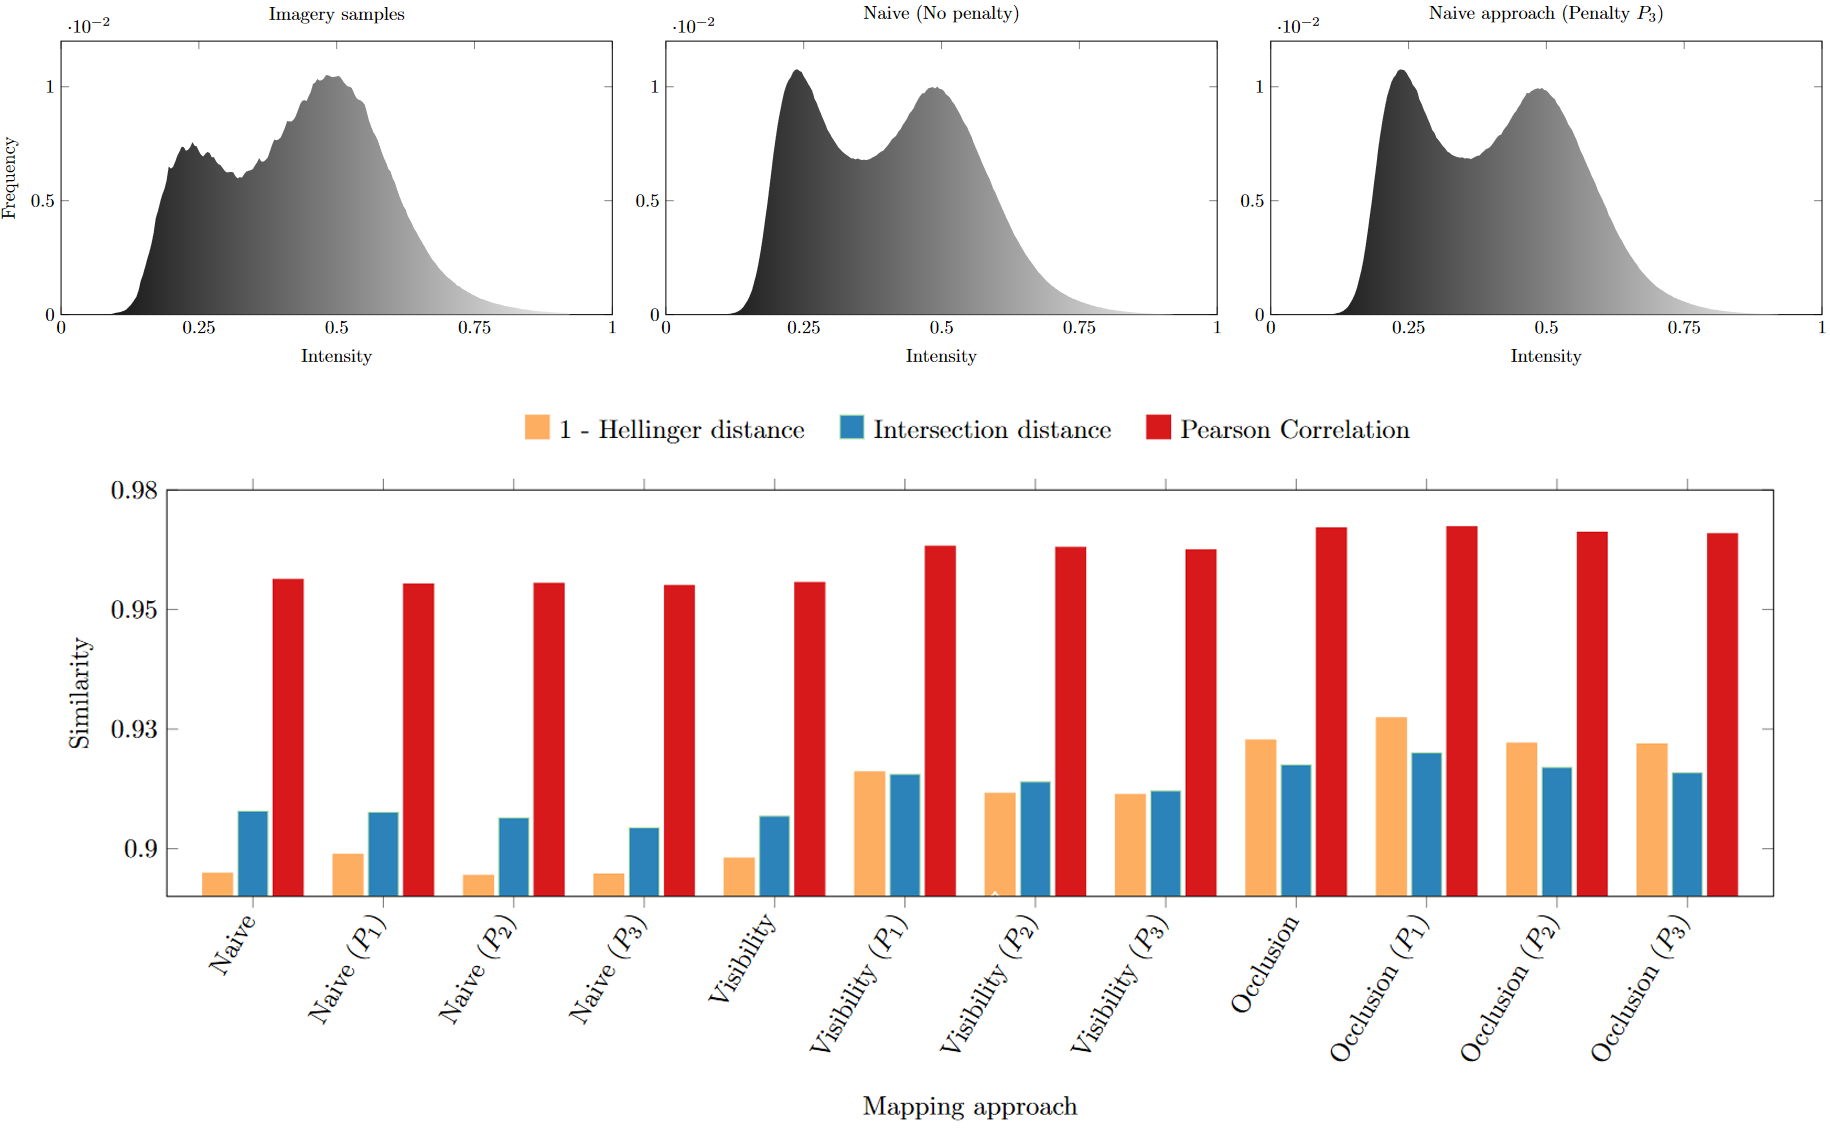
\includegraphics[width=.9\linewidth]{figs/thermal_projection/histogram_composition.png}
% 	\caption{Intensity distribution for image samples collected in the reconstruction of a thermal point cloud, as well as the grayscale distribution obtained after applying naive (no penalty) and naive (penalty-based, $P_3$) approaches. The density functions concerning other variants were omitted as they returned very similar results. Finally, the similarity between histograms was reported for each configuration, with minor changes in the distribution being highlighted. For the sake of clarity, Hellinger distance was expressed as $1 - d$ to visualize the three metrics in the same chart. Hence, a value of 1 indicates that both histograms are equal ($h_{1_{i}} = h_{2_{i}}, \forall i \in [0, n)$), while 0 denotes complete dissimilarity ($h_{1_{i}} = 1 - h_{2_{i}}, \forall i \in [0, n)$).}
% 	\label{fig:thermal_histogram_results}
% \end{figure*}

Figure \ref{fig:thermal_histogram_results} compares the source histogram for the naive approach and the histograms obtained from by mapping thermal data with no penalty function and using the penalty function $P_3$. The rest obtained similar results and thus were omitted in this comparison. These small variations are more clear in Figure \ref{fig:thermal_histogram_results}. Remark that $d_{\textit{hellinger}}$ was transformed into $1 - d_{\textit{hellinger}}$ to make all of the distance functions fall in the same interval. According to the results, occlusion-based mapping obtained more similar results to the baseline histogram, especially using the occlusion test. Furthermore, the penalty function $P_1$, which computes the dispersion as $\abs{x_i - y}$, had better results for every approach.

\newpage
\subsection{Analysis of thermal point cloud}

\begin{marginfigure}[1cm]
	\centering
	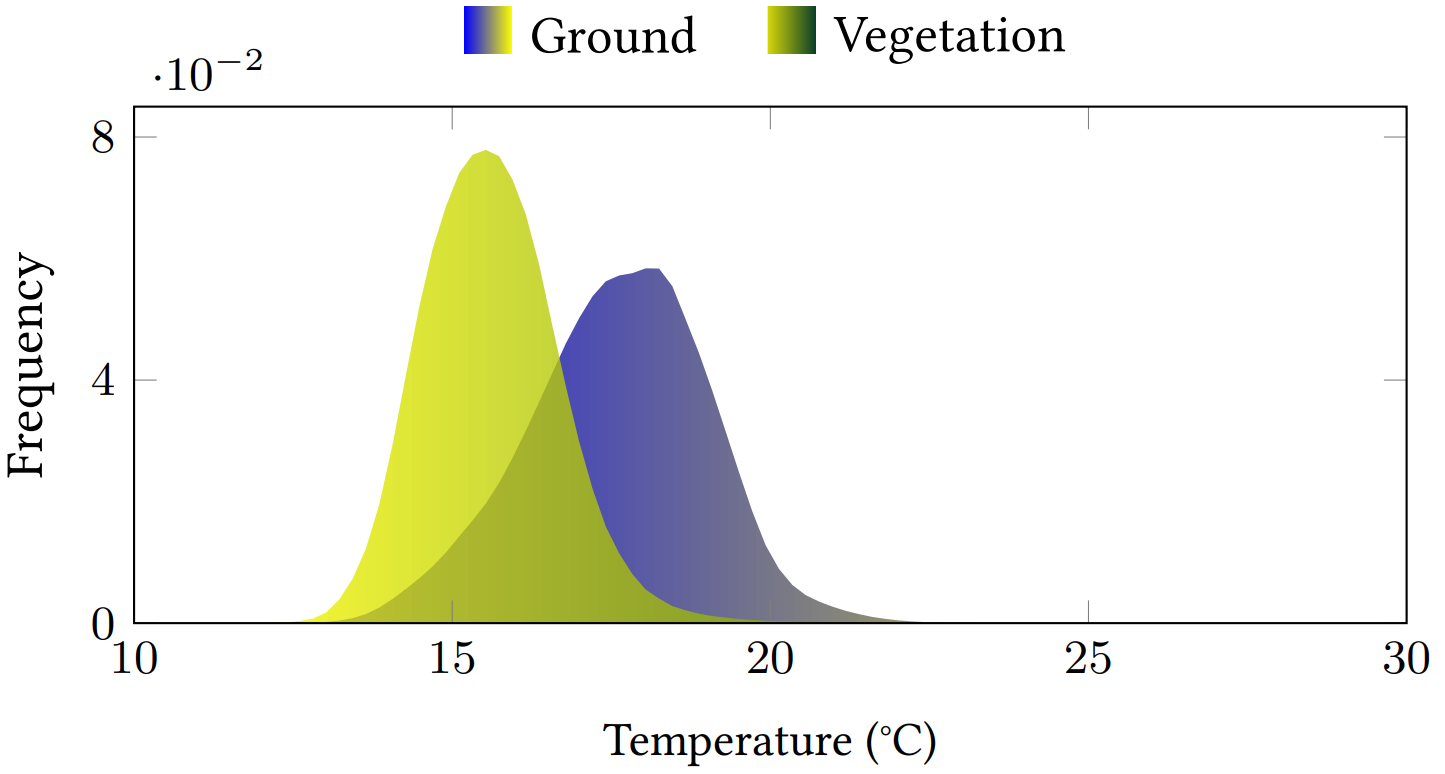
\includegraphics{figs/thermal_projection/temperature_class.png}
	\caption{Frequency diagram of thermal radiation for 3D points labelled as ground and vegetation.}
	\label{fig:thermal_temperature_class}
\end{marginfigure}
The temperature collected from ground and vegetation points is depicted in Figure \ref{fig:thermal_temperature_class}, using a point cloud of nearly 100M points. Accumulated values are presented as a density function based on the point cloud size. Although Figure \ref{fig:thermal_temperature_class} shows that vegetation presents overall less emission of thermal radiation, both datasets are far from being disjoint. It is worth noting that the vegetation label also comprises dry weeds which were classified as anomalous hot regions. On the other hand, ground points also cover regions shadowed by trees. However, the local maxima of both thermal distributions clearly yield a relevant value for our two categories. Most thermal values range from 12 \textdegree C to 23 \textdegree C; anomalous hot regions are detected in vegetation and metal surfaces, whereas cold regions are located at isolated trees and ground points.

\subsection{Visualization of the point cloud}

A better insight into the reconstructed point clouds is provided by Figure \ref{fig:thermal_point_cloud_comparison}. It depicts three results (b, c and d): the first one is computed using the naive approach, while the other two are the outcome of Agisoft Metashape and Pix4Dmapper software. It is worth noting that Pix4Dmapper utilizes a different grayscale distribution, as the software is capable of extracting absolute thermal values from the image dataset. Therefore, such values are normalized considering the minimum and maximum temperatures. As shown in Figure \ref{fig:thermal_point_cloud_comparison}, the result of Pix4Dmapper presents empty regions which correspond to images that could not be calibrated. Furthermore, canopies were poorly estimated and appear much noisier than in the \acrshort{rgb} reconstruction, which is
known to be geometrically accurate. Also, trees present a higher elevation in comparison with the \acrshort{rgb} point cloud. 

Regarding the result of Agisoft Metashape, it presents a wide number of relevant errors. First, canopies were badly estimated, to the extent that they are represented as planar surfaces and show visible outliers. Furthermore, a significant part of the study area is placed several meters below the rest of the environment. Finally, sparsity concerns both point clouds, although it is more significant in the Pix4Dmapper result, as reported in Table \ref{table:thermal_point_cloud_approaches}. Finally, the preservation of details is proved acquired in Figure \ref{fig:thermal_zoomed_up}, where neither blurring nor distortion effects are visible. The corrections, projection and aggregation operators enabled the reconstruction of a thermal point cloud with a geometry provided by the baseline RGB point cloud.

\begin{figure*}[hbt]
	\centering
    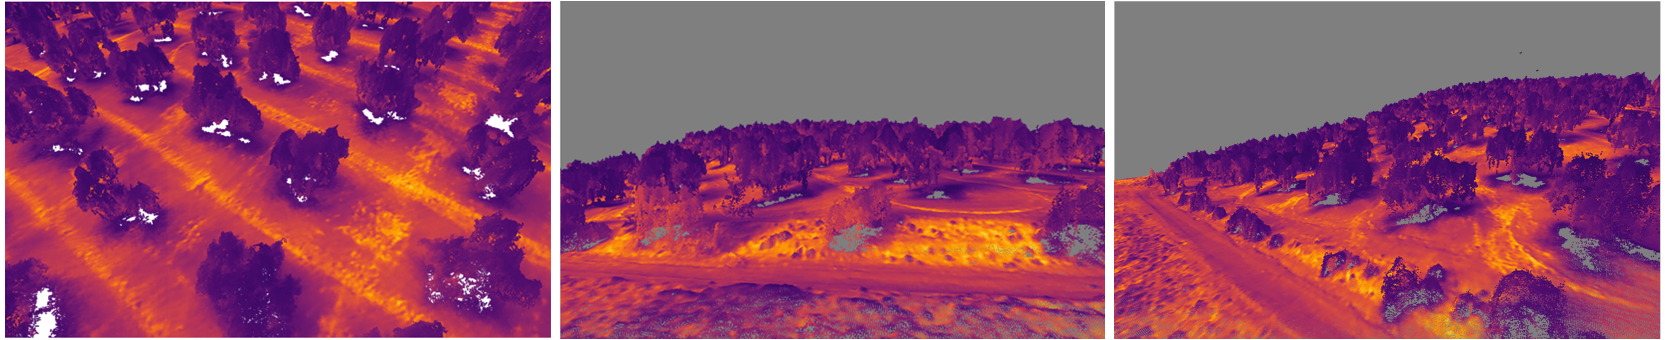
\includegraphics[width=\linewidth]{figs/thermal_projection/thermal_close_view.png}
	\caption{Close-up view of a thermal point cloud with $\sim20$ million points. Details of thermal images are preserved and no blurring effects are observed.}
	\label{fig:thermal_zoomed_up}
\end{figure*}

\section{Conclusions and future work}
\label{Conclusions and future work}

An efficient algorithm for building dense \acrshort{tir} point clouds was proposed in this chapter. \acrshort{rgb} point clouds were used as the input for generating an output with a larger number of points (up to 798.69\% more points than commercial software). \acrshort{gpu}-based algorithms were used to fasten some of the proposed algorithms, thus obtaining a decrease of 78.39\% in the processing time per 3D point in comparison with Agisoft Metashape. An innovative solution for the aggregation of multiple thermal samples was also proposed to minimize the dissimilarity of thermal values in 3D points and image intensity. Dispersion and histogram distance metrics showed that penalty functions clearly help in this task.

\begin{figure*}[htb]
    \centering
    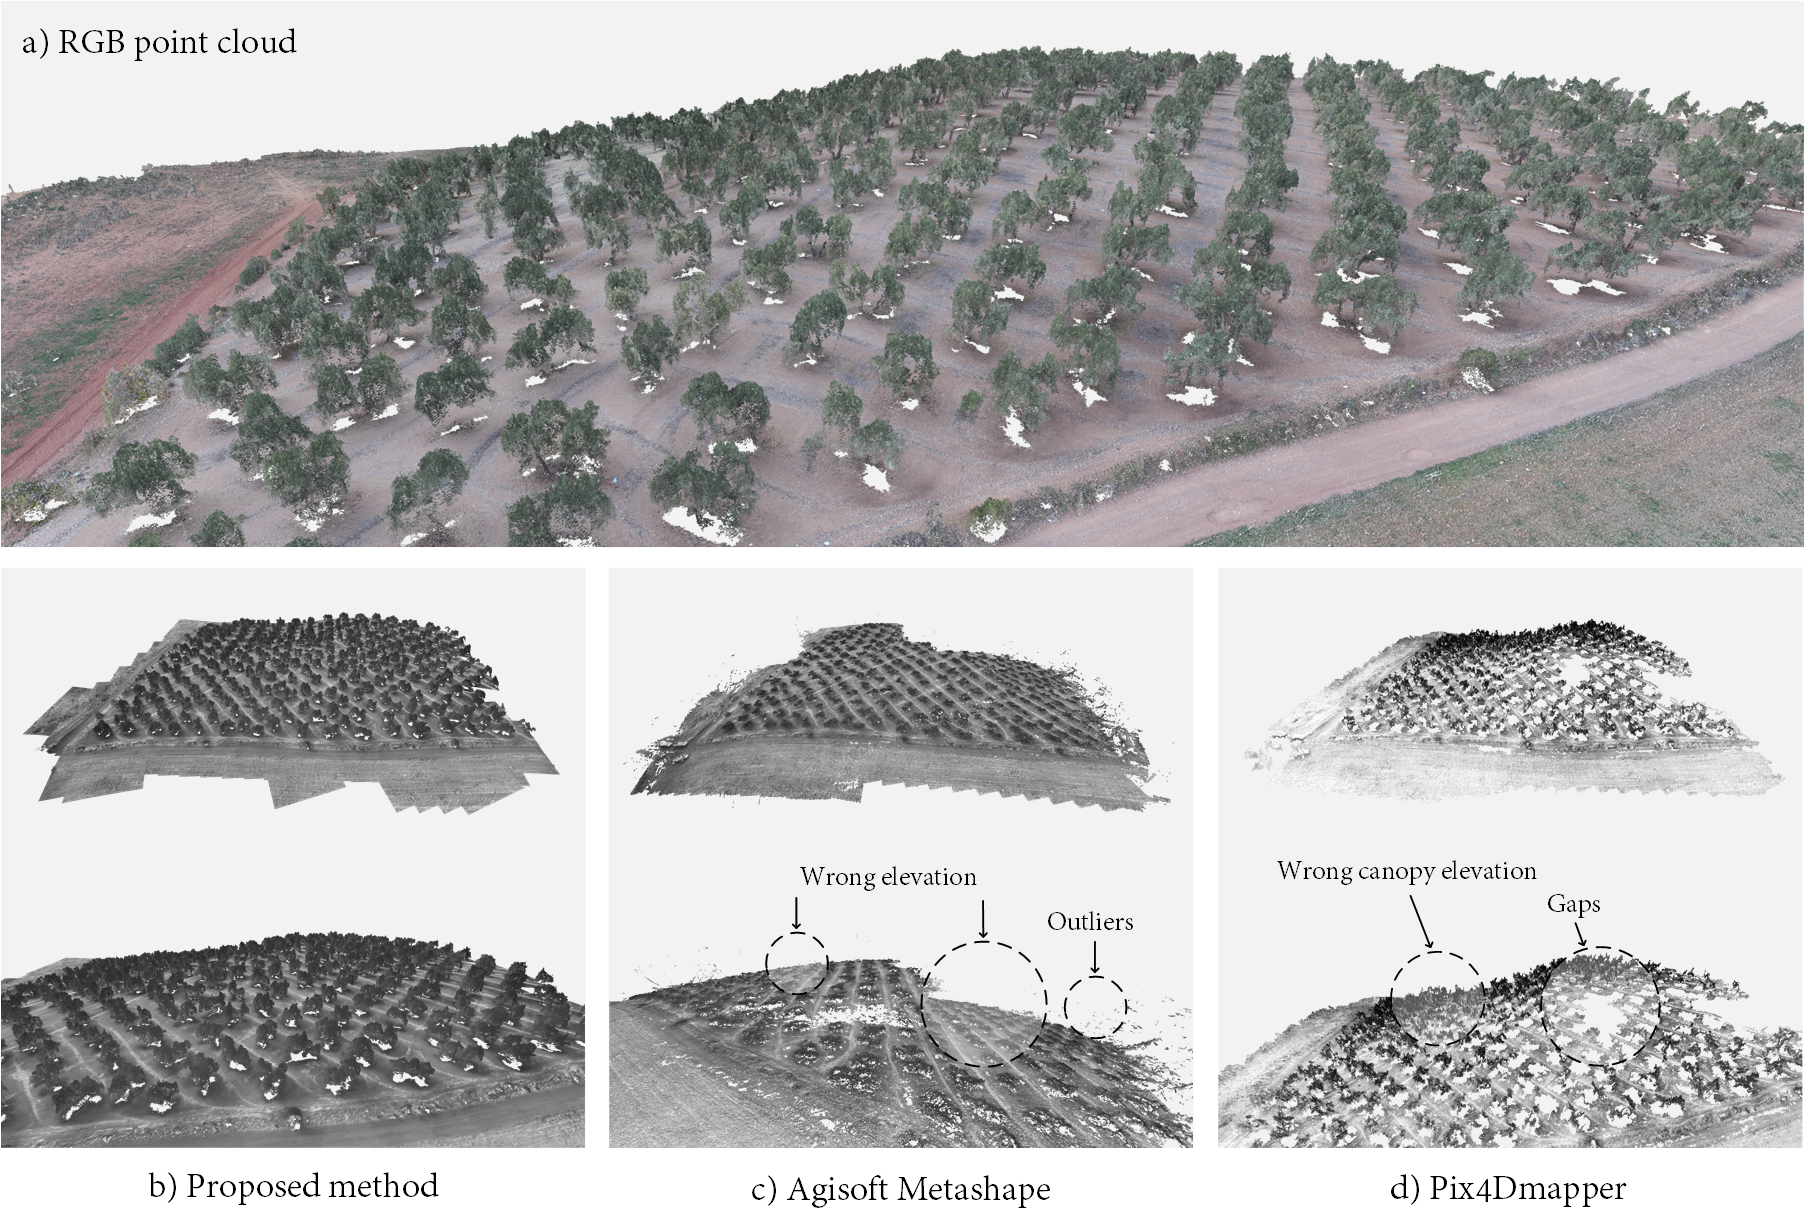
\includegraphics[width=\linewidth]{figs/thermal_projection/thermal_visualization_comparison.png}
	\caption{a) Original \acrshort{rgb} point cloud, retrieved with the original resolution, b) thermal point cloud computed using the naive approach, c) Agisoft Metashape result and 4) Pix4Dmapper result. }
	\label{fig:thermal_point_cloud_comparison}
\end{figure*}

This methodology is appropriate as an alternative to the traditional \acrshort{sfm}-\acrshort{mvs} algorithm. The latter is based on extracting features from images, which are harder to obtain from thermography. Instead, the \acrshort{rgb} point cloud generated by \acrshort{sfm} can be used as the baseline for projecting imagery. Also, the density of the point clouds estimated by our algorithm was higher and thus it could be more suitable for applications that require dense results, e.g., rendering software. Similarly, it operates as an efficient solution that helps in reducing latency.

\marginnote[-2cm]{The \acrshort{ecc} image matching can be barely improved from here. However, the acquisition of thermal images was performed so that visual information is obtained by fusing infrared and \acrshort{rgb} data. Although it may help on some datasets, the included edges were very fuzzy for vegetation. Hence, disabling this overlapped data may help in the image-matching task. } 
This chapter leaves some open questions that will be addressed in later chapters or remains as future work. Firstly, in-situ radiometric calibration may help on shedding light on the accuracy of the temperature estimation. From here, a reliable multi-temporal system could be proposed over reconstructed thermal point clouds for the analysis of individual trees. As previously stated, the target area was partly affected by the \textit{Xylella fastidiosa} pathogen and thus could be monitored using thermography. The registration of \acrshort{rgb} and thermal images could also be improved to increase the point density of resulting point clouds. Finally, more competitive solutions concerning efficiency could be developed by implementing the entire workflow in \acrshort{gpu}, which is the topic of the following chapter. This study could be further extended to compare several parallel-computing frameworks and take advantage of rendering tools, such as OpenGL's built-in \textit{z}-buffer.